
\documentclass[a4paper,11pt]{book}
\usepackage{etex}

\reserveinserts{28}


%%%%%%%%%%%%%%%%%%%%%%%%%%%%%%% PACKAGES %%%%%%%%%%%%%%%%%%%%%%%%%%

\usepackage[english]{babel}
\usepackage{algorithm}
\usepackage{algpseudocode}
\usepackage{amsmath,amssymb,amscd,mathtools,amstext,amsthm}
\usepackage{stmaryrd}
\usepackage{soul}
\usepackage{setspace} % For \setstretch
\usepackage[nomessages]{fp} % for FPval, etc.
\usepackage{amsmath}
\usepackage{multirow}
\usepackage{tikz}
\usetikzlibrary{arrows}
\usepackage{xcolor}
\usepackage{array}
\usepackage{tabularx}
\usepackage{ctable}
\usepackage{multirow}
% \usepackage{subfigure}
\usepackage[colorlinks=false,hidelinks]{hyperref}
\usepackage[nameinlink]{cleveref}
\usepackage{balance}
\usepackage{xspace}
\usepackage{paralist}
\usepackage{longtable}
\usepackage[flushleft]{threeparttable}
\usepackage{epsfig}
\usepackage{subfigure}
\usepackage{lettrine}
\usepackage{bibentry}
\usepackage{enumitem}
\usepackage[all]{nowidow}
\usepackage{mytitlesec}
\usepackage{fancyhdr}
\usepackage{minitoc}
\usepackage{csquotes}
\usepackage[final]{pdfpages}
\usepackage{xcolor,colortbl}
\doparttoc

%%%%%%%%%%%%%%%%%%%%%%%% REDEFINITION OF CHAPTER

\titleformat
{\chapter} % command
[display] % shape
{\bfseries\Huge} % format
{Chapter \thechapter} % label
{0.5ex} % sep
{
    \rule{\textwidth}{1pt}
    \huge
    % \vspace{1ex}
} % before-code
[
\vspace{-0.5ex}%
\rule{\textwidth}{1pt}
] % after-code



 
%%%%%%%%%%%%%%%%%%%%%%%% REDEFINITION OF PAGE STYLE
\fancyhf{}
\fancyhead[RE,LO]{\thesisTitle}
\fancyhead[LE,RO]{Dinh T.Van}
\fancyfoot[CE,CO]{\thepage}



\newcommand*\circled[1]{\tikz[baseline=(char.base)]{
            \node[shape=circle,draw,inner sep=.6pt] (char) {#1};}}

%url
\def\UrlBreaks{\do\.\do\ \do\\\do\/\do\!\do\_\do\|\do\%\do\;\do\>\do\]
\do\)\do\,\do\?\do\'\do\+\do\=\do\#\do\-}%
\Urlmuskip=0mu plus 1mu %





\newcommand{\thesisTitle}{Kernel-based methods for Graph-based Data Integration}

%%%%%%%%%%%%%%%%%%%%%%%%%%%% GLOBAL

\newcommand{\HRule}{\rule{\linewidth}{0.2mm}}
\newcommand{\bigO}[1]{\ensuremath{\mathcal{O}(#1)}\xspace}
\newcommand{\bitstring}[1]{#1}
\renewcommand{\paragraph}[1]{\hfill\\\noindent{\bf#1}}
\newcommand{\newpar}[1]{\hfill\\\noindent{\bf#1}}


%%%%%%%%%%%%%%%%%%%%%%%%%%%%5 Math
\newcommand{\norm}[1]{\left\lVert#1\right\rVert}
\newcommand{\tr}{^\mathsf{T}}
\setcounter{secnumdepth}{3}
\setcounter{tocdepth}{4}
\setcounter{secnumdepth}{4}

\newtheorem{theorem}{Theorem}
\usepackage{xcolor}
\usepackage{hyperref}
\theoremstyle{definition}
\newtheorem{definition}{Definition}[section]
\usepackage{pdflscape}
\usepackage{setspace}
\usepackage{amsmath}
\usepackage[toc,page]{appendix}
\linespread{1.1}

\makeatletter
\setlength{\@fptop}{0pt}
\makeatother


\hypersetup{
    colorlinks=true,
    linkcolor=blue,
    filecolor=magenta,      
    urlcolor=cyan,
    pdftitle={Sharelatex Example},
    bookmarks=true,
    pdfpagemode=FullScreen,
}


\begin{document}

\sloppy

\pagenumbering{roman}
\pagestyle{plain}
\begin{titlepage}
	%\begin{adjustwidth}{-1cm}{0.1cm}
	\begin{center}
	
		
\includegraphics[width=4.5cm]{img/logoUnipd.png}

		
		\vspace{.5cm}
		\textrm{\LARGE University of Padua}
		\\[.1cm]
		\textrm{\Large Department of Mathematics\xspace}
		\\[.1cm]
		\textrm{\normalsize Doctorate Degree in Brain, Mind and Computer Science}
		\\[.1cm]
		\textrm{Curriculum in Computer Science}\\
		
		\vspace{.5cm}

		
		\vspace{1cm}
		
		% Title
		\HRule \\
		\vspace{.5cm}
		\scshape{\large \textbf{ KERNEL METHODS FOR LARGE-SCALE} \\[0.25cm]
		\textbf{ GRAPH-BASED HETEROGENEOUS BIOLOGICAL} \\[0.25cm] \textbf{ DATA INTEGRATION}}\\
		\vspace{.4cm}
		
		\HRule\\
		\vspace{3cm}
		
		% % Author and supervisor
		% \begin{minipage}{0.5\textwidth}
		% 	\begin{flushleft} \large
		% 		\textbf{Candidate:}\\
		% 		Moreno Ambrosin	
		% 	\end{flushleft}
		% \end{minipage}
		% \begin{minipage}{0.4\textwidth}
		% 	\begin{flushright} \large
		% 		\emph{Supervisor:} \\
		% 		Dott.sa Crafa Silvia
		% 	\end{flushright}
		% \end{minipage}
		{\centering
		\begin{tabular}{ l c r }
			{\large{\bf Candidate}}					& \hspace{90pt} 					& {\large{\bf Supervisor}}\\
			\textrm{\large Dinh Tran Van}						&				 					& \textrm{\large Prof. Alessandro Sperduti} \\
													&				 					& {\em University of Padova, Italy}\vspace{5mm}\\
			 				&				 					& \\
							&									& \\
													&									& \\
		\end{tabular}
		}
		\vfill
		
		% Bottom of the page
		%{\large Octobor 31\textsuperscript{st}, 2017}
		\today
		
	\end{center}
	%\end{adjustwidth}
\end{titlepage}
\chapter*{Acknowledgments}
Firstly, I would like to express my sincere gratitude to my advisor Prof. Alessandro Sperduti for the continuous support of my Ph.D study, for his patience, motivation and enthusiasm.


Besides my advisor, I would like to thank the rest of my thesis committee for their insightful and valuable comments and suggestions.


I would like to thank Dr. Alberto Testolin for all his help and for his guidance before and during my Ph.D studies.  Also, I would like to thank Prof. Peter Tino for the meaningful discussions and inputs he provided during my visit to University of Birmingham.


I would like to thank all my friends, colleagues and officemates (Moreno, Riccardo, Alberto, Daniele, Hossein and Ding Ding) here at the University of Padua for the stimulating discussions, and for all the fun we have had in the last three years.


Last but not the least, a huge thank goes to my family, that always supported me in these years. Words cannot express how grateful I am to my mother, and father for all of the sacrifices that they have made on my behalf.
\vspace{2cm}
\begin{flushright}
Dinh Tran Van~~~~~\\
Padova, \today ~~~~~
\end{flushright}
\chapter*{Abstract}
We have been witnessing the explosive growth of biological data in terms of volume and variety, thanks to the development of technologies related to web services and embeded systems. Such data can naturally be represented as graphs. It is common that entities are encoded in different data sources. On the one hand, this provides a great opportunity for us to have unified views about entities of interest. On the other hand, this poses challenges for scientists to wisely extract knowledge from such huge amount of data which normally cannot be done without the help of automated learning systems. Therefore, there is a need of developing smart learning systems which support experts to form and assess hypotheses in biology and medicine. The problem of data integration in general or graph-based data integration in specific needs to be efficiently solved if we desire to build high performance learning systems. The contributions of this thesis focus on addressing challenges for graph-based data integration problem with the aim of achieving high performance systems: \textit{node similarity measure}, \textit{graph sparsity}, \textit{scalability}, \textit{effectiveness and efficiency}.\\

The first contribution is the definition of an efficient graph node kernel named Conjunctive disjunctive graph node kernel which aims at defining the similarity between any graph node couple. The kernel first decomposes the input graph into a collection of connected sparse graphs. It then develops a suitable kernel that explicitly models the configuration of each node's context to measure node proximity. The proposed kernel shows state of the art performance for graph node kernels.\\

The second contribution of this thesis aims to deal with graph sparsity problem by introducing a link prediction method whose objective is to enrich links of a graph. In this method we first represent each link connecting two nodes by a graph composed of their neighborhood subgraphs. We then cast the link prediction problem as a binary classification task over obtained graphs in which we employ an efficient decompositional graph kernel for graph similarity. Empirical evaluation proves the promissing of the method.\\

The third contribution is a proposed method to enrich the performance of diffusion-based graph node kernels when working with sparse graphs caused by the lack of information. By adding link enrichment phase before employing diffusion-based kernels, we empirically show a robust and large effect for combination of a number of link prediction and a number of diffusion-based kernels on several real gene-disease association problems.\\

The fourth contribution copes with the scalability problem by proposing scalable kernel-based gene prioritization method (Scuba). Scuba is optimized to deal with strongly unbalanced setting and is able to deal with both large amount of candidate genes and arbitrary number of data sources. It outperforms and enhances the scalability, efficacy comparing with existing methods for disease gene prioritization.\\

The last contribution is an approach for graph integration targeting to solve disease gene prioritization problem. In this method, the common genes between graph layers, derived from biological sources, are connected by disjunctive links. Then a particular graph node kernel is adopted to exploit topological graph features from all layers for measuring gene similarities. The state of the art performance on different experimental settings confirms the strength of the method. 

\cleardoublepage
\cleardoublepage

\tableofcontents

\cleardoublepage

%*******************************************************
% Mainmatter
%*******************************************************
\pagenumbering{arabic}
\pagestyle{fancy}
\cleardoublepage
\chapter{Introduction}
\section{Graph-based Data Integration}
\section{Challenges}
	\subsection{Node Similarity Measure}
	\subsection{Sparsity}
	\subsection{Scalability}
	\subsection{Effectiveness and Efficiency}
\section{State of the Art Graph-based Data Integration}
\section{Contributions}
\subsection{Conjuctive Disjuctive Graph Node Kernel}
\subsection{Joint Neighborhood Subgraphs for Link Prediction}
\subsection{Link Enrichment for Diffusion-based Graph Node Kernels}
\subsection{Scalable Kenrel-based Gene Prioritization}
\subsection{Disjunctive Interconnection Graphs for Disease Gene Prioritization}
\chapter{Background}
\label{chap:background}
In this chapter, we describe preliminary knowledge and notaions used for the remaining parts of this thesis to make it easy for readers to follow.
\section{Machine Learning}
Recently, \textit{machine learning} has become a must-know term not only in academia but also in daily life due to the popularity of it's applications in various fields. Machine learning can be considered as a branch of Artificial Intelligence which aims at providing systems the ability to automatically adapt to their environment and learn from experience without being explicitly programmed. According to \cite{mitchell1997machine}, machine learning is formally defined as:

\begin{definition}{}
\textit{A computer program is said to learn from experience $E$ with respect to some task $T$ and some performance measure $P$ if its performance on $T$, as measured by $P$, improves with experience $E$.}
\end{definition}

We denote $\mathbb{X}$ as domain dataset which encodes the complete information of a domain. For each domain, however, we are only able to collect a small fraction of domain dataset, $\mathbb{D}$, resulted from any observation, measurement or recording apparatus such that $\mathbb{D} \cup \mathbb{X}$. The set $\mathbb{D}$ is normally referred as the training dataset. Machine Leanring techniques desire to exploit $\mathbb{D}$ to get useful information for constructing a model that generalizes nature of data source. The model is then used to make prediction or inference in unseen dataset, $\mathbb{U} = \mathbb{X} - \mathbb{D}$.

Machine Learning algorithms can be classified into three groups: supervised learning, unsupervised learning and reinforcement learning. Supervised learning proceed with datasets whose objects are associated to labels, while unsupervised learning works with datasets consisting of input data without labeled responses. Reinforcement Learning aims at designing machines and software agents that can automatically determine the ideal behaviour within a specific context, in order to maximize its performance. Simple reward feedback is required for the agent to learn its behaviour; this is known as the reinforcement signal. In this thesis, we focus on supervised learning scenario. 

We consider a training set $\mathbb{D}$ generated by an unknown probability distribution $\mathcal{P}$,  $\mathbb{D} = \lbrace (x_1, y_1), (x_2, y_2),\ldots, (x_n, y_n)  \rbrace$ where $x_i \in \mathbb{X}$ are examples and $y_i \in \mathbb{Y}$ are labels. The relations between $x_i$ and $y_i$ are defined by a true function (target function) $f: \mathbb{X}\longmapsto \mathbb{Y}$. What we desire to do is to learn the function $f$. However, the only information we can access is from the training set. Therefore, a supervised learning method aims at estimating a function $g$ based on $\mathbb{D}$ to be as close to $f$ as possible. Depending on the domain of $\mathbb{Y}$, we can further group supervised learning methods into following sub-groups:
\begin{itemize}
	\item if $\mathbb{Y} \subseteq \mathbb{R}$, the problem is called regression
	\item if $\left\vert{\mathbb{Y}}\right\vert = 2$, we have a binary classification problem
	\item if $\left\vert{\mathbb{Y}}\right\vert = n$ with $n>2$, we have multi-class classification problem
\end{itemize}
Besides, a supervised learning algorithm is called multi-labels classification if an example could have more than one label associated with that. It is worth highlighting that there is normally more than one possible choice for $g$. We refer each choice of $g$ as a hypothesis ($h$) or model and the set of all possible $g$ as hypothesis space, $\mathbb{H}$. A hypothesis space need to be define in advance and it is necessary to contains good approximations to target function. In order to find the optimal hypothesis, $h^*$, one way is to employ a true loss function, $\mathcal{L}$, which measures how much a hypothesis fails to correctly map between examples and their corresponding labels.
\begin{equation}
\label{loss-function}
\mathcal{R}(h) = \int_{\mathbb{X}\times \mathbb{Y}}^{} \mathcal{L}(h(x),y)dP(x,y)
\end{equation}
The optimal function with the least of mis-mappings (errors) is then the solution of following optimization:
\begin{equation}
\label{opt-loss-function}
h^{*} = \arg\min_{h \in \mathbb{H}}\mathcal{R}(h)
\end{equation}
Unfortunately, it is impossible to directly solve the optimization \ref{loss-function} since the probability distribution $\mathcal{P}$ in the true loss function \ref{opt-loss-function} is an unknown function and we only have access to a finite training set $\mathbb{D}$. In this case, an alternative approach is to use empirical loss instead of true loss function. The empirical loss function is defined over the training set as follow:
\begin{equation}
\mathcal{R}_{emp}(h) = \frac{1}{n} \sum_{n=1}^{n} |h(x_i) - y_i| 
\end{equation}
However, in order to use $\mathcal{R}_{emp}(h)$, we need to guarantee that the value of $\mathcal{R}_{emp}(h)$ converges to the value of $\mathcal{R}(h)$?. Using the law of large numbers, authors prove in \cite{vapnik1998statistical} that the convergence happens when the number of examples is high enough. For more details we refer the reader an amazing book \cite{vapnik1998statistical}.
\section{Kernel Methods}
\label{kernel-methods}
In classical machine learning techniques for binary classification, first the data presentation form is defined, strings, vectors for instances. It then is used to represent for each example, $x\in\mathbb{X} \longrightarrow \phi(x) \in \mathbb{F}$. After a linear function is learnt to separate positive examples from negative ones. Although these approaches have sucessfully applied in some cases, they share two common limitations: \textit{i}) the high comlexity when working with high dimensional spaces. \textit{ii}) the difficulty or impossiblity to find the vectorical form to represent data in many cases.

Recently, a new framework named Kernel method has been proposed and shown the state-of-the-art results in many cases of various fields. SVM \cite{cortes1995support} is a typical example of kernel methods. Unlike the presentation of data in traditional machine learning, data are not individually represented in kernel methods, but through a set of pairwise similarities. More precisely, a matrix whose each element is a real-valued comparision between two examples is used to represent for a data set. These real-valued elements are computed by using a kernel function: $k: \mathbb{X} \times \mathbb{X} \longmapsto \mathbb{R}$. By using matrix to represent for data set, the presentation of data in kernel methods does not depend on the nature of objects. That means the presentation of strings, images,\ldots are the same. More interesting, it allows kernel machines to modularize into two components: the design of a specific kernel function and the design of a general learning algorithm (kernel machine).
\section{Kernel functions}
As stated in \ref{kernel-methods}, in kernel methods, the definition of kernel functions is independent from the definition of general learning algorithms. Therefore, it provides kernel machines more options when employing kernels. A number of kernel functions have been proposed for different types of data. In this section, we first formally define what is a kernel function. We then introduce some kernels defined on graphs that later on are used in our experiments.
\begin{definition}{}
\textit{Given a set of object $\mathbb{X}$, a function $k: \mathbb{X} \times \mathbb{X}\longmapsto \mathbb{R}$ is called a kernel on $\mathbb{X} \times \mathbb{X}$ iff $k$ is
\begin{itemize}
	\item symmetric: it means $k(x_1,x_2) = k(x_2,x_1)$, where $x_1, x_2 \in \mathbb{X}$.
	\item positive semi-definite: that is
	$\sum_{i=1}^{N}\sum_{j=1}^{N}c_ic_jk(x_i,x_j) \geq 0$ for any $N>0$, $c_i, c_j \in \mathbb{R}$, and  $x_i, x_j \in \mathbb{X}$.
\end{itemize}
}
\end{definition}
A kernel is usually represented as a matrix $K$ which is called Kernel matrix (Gram matix) and $K$ needs to be symmetric, i.e. $K(x_1,x_2) = K(x_2,x_1)$, positive semi-definite, i.e. its eigen values are non-negative. In this thesis, kernels and kernel matrcies are identical. 

One of the most simple kernel called Linear kernel which is defined on vectors, $\mathbb{X} \subseteq \mathbb{R}^n$. $k_L(x_1, x_2) = x_{1}^\intercal x_2$, where $x_1, x_2 \in \mathbb{X}$. This kernel suggests a systematic way to define kernels. Given a general set of object $\mathbb{X}$, we first project each element in $\mathbb{X}$ into a vector space, $x \in \mathbb{X} \longrightarrow \phi(x) \in \mathbb{R}^n$. Next, we define a kernel as:
\begin{equation}
k(x_1, x_2) = \phi(x_1)^\intercal \phi(x_2)
\end{equation}
Interestingly, any kernels defined on $\mathbb{X}$, there exists a Hilbert space, $\mathbb{F}$ and a mapping $\phi: \mathbb{X}\longrightarrow \mathbb{F}$ such that $k(x_1, x_2)= \langle \phi(x_1),\phi(x_2) \rangle$, where $x_1, x_2 \in \mathbb{X}$.

There are two problems we might face with if we would like to explicitly embed objects into a vector space. \textit{i}) We need to deal the high computation if we embed objects into high demensional spaces. \textit{ii}) We do not have clear way to represent objects in vectorial forms. These limitations are effectively solved by using \textit{Kernel trick}. The kernel trick avoids the explicit mapping. Instead, it allows the operations (dot product) between vectors in the feature space to be done by computing only in the input space.

A kernel is considered as a similarity (proximity) measure since its value computed for two objects is proportional to their similarity.

Most kernels are defined on vectorial form of data in which Radial basis function kernel (RBF) \cite{vert2004primer} is the most used one. However, real world data often cannot be represented in the vectorial form without lossing important information. Therefore, a high number of kernels are proposed to deal with structured data, including trees, graphs, etc. 

In many domains, relational data can be naturally represented by graphs (networks) whose nodes are entities and links characterize relations between entities. One example is the gene network where each node represents for a gene and each link is formed between two genes if they encode common protein(s). Another example is the social network whose nodes are users and links depict friendship between users. There are many systems have been proposed that take graphs as their input. These systems can be called as graph-based systems. One of the key points that determines the performance of graph-based systems is the definition of node similarity measure. Graph node kernels are popular and most used to measure the proximity between nodes of a graph. Following, we first give a formal definition of a graph as well as graph related definitions and notations. We then briefly describe kernels defined on graphs. Kernels on graphs could be designed on vertices of graphs or between graphs. We refer kernels in the former case as graph kernels and the latter one as graph node kernels.
\begin{definition}{}
\textit{A graph, notated as $G = \left(  \mathbb{V}, \mathbb{E} \right)$, is a structure which consists of a set of nodes (vertices), $V = \lbrace v_1, v_2,\ldots, v_n\rbrace$, and a set of links (edges), $\mathbb{E} = \lbrace (v_i, v_j)\rbrace \subseteq (\mathbb{V}\times \mathbb{V})$.}
\end{definition}

\begin{definition}{}
\textit{An adjacency matrix $\textbf{A}$ is a symmetric matrix used to characterize the direct links between vertices $v_{i}$ and $v_{j}$ in the graph. Any entry $A_{ij}$ is equal to 1 when there exists a link connecting $v_{i}$ and $v_{j}$, and is 0 otherwise.}
\end{definition}

\begin{definition}{}
\textit{The Laplacian matrix $\textbf{L}$ is defined as $\textbf{L} = \textbf{D}-\textbf{A}$, where $\textbf{D}$ is the diagonal matrix with non-null entries equal to the summation over the corresponding row of the adjacency matrix, i.e. $\textbf{D}_{ii}=\sum_j \textbf{A}_{ij}$.}
\end{definition}
\subsection{Graph Kernels}

\subsection{Graph Node Kernels}
It is different from graph kernels which aims at measuring similarities between graphs, graph node kernels intend to measure proximities between nodes in graphs. In the following, we introduce some of the most used graph node kernels.
\subsubsection{Laplacian exponential diffusion kernel}
One of the most well-known kernels for graphs is the Laplacian exponential diffusion kernel \textbf{LEDK}, as it is widely used for exploiting discrete structures in general and graphs in particular. On the basis of the heat diffusion dynamics, Kondor and Lafferty proposed \textbf{LEDK} in \cite{kondor2002diffusion}: imagine to initialize each vertex with a given amount of heat and let it flow through the edges until an arbitrary instant of time. The similarity between any vertex couple $v_{i}$, $v_{j}$ is the amount of heat starting from $v_{i}$ and reaching $v_{j}$ within the given time. Therefore, \textbf{LEDK} can capture the long range relationship between vertices of a graph to define the global similarities. Below is the formula to compute \textbf{LEDK} values:
\begin{equation} 
\label{LEDK-formula}
K = e^{-\beta \textbf{L}} = \textbf{I} - \beta \textbf{L} + \frac{\beta \textbf{L}^{2}}{2!} - ...
\end{equation}
where $\beta$ is the diffusion parameter and is used to control the rate of diffusion and $\textbf{I}$ is the identity matrix. Choosing a consistent value for $\beta$ is very important: on the one side, if $\beta$ is too small, the local information cannot be diffused effectively and, on the other side, if it is too large, the local information will be lost. \textbf{LEDK} is positive semi-definite as proved in \cite{kondor2002diffusion}.
\subsubsection{Exponential diffusion kernel}
In \textbf{LEDK}, the similarity values between high degree vertices are generally higher compared to those between low degree ones. Intuitively, the more paths connect two vertices, the more heat can flow between them. This could be problematic since peripheral nodes have unbalanced similarities with respect to central nodes. In order to make the strength of individual vertices comparable, a modified version of \textbf{LEDK} is introduced by Chen et al in \cite{chen2014disease}, called Markov exponential diffusion kernel \textbf{MEDK} and given by the following formula:
\begin{equation} \label{MEDK-formula}
\textbf{K} = e^{-\beta \textbf{M}}
\end{equation}
The difference with respect to the Laplacian diffusion kernel is the replacement of \textbf{L} by the matrix $\textbf{M}=(\textbf{D}-\textbf{A}-n\textbf{I})/n$ where $n$ is the total number of vertices in graph. The role of $\beta$ is the same as for \textbf{LEDK}.
\subsubsection{Markov diffusion kernel}
The original Markov diffusion kernel \textbf{MDK} was introduced by Fouss et al. \cite{fouss2006experimental} and exploits the idea of diffusion distance, which is a measure of how similar the pattern of heat diffusion is among a pair of initialized nodes. In other words, it expresses how much nodes "influence" each other in a similar fashion. If their diffusion ways are alike, the similarity will be high and, vice versa, it will be low if they diffuse differently. This kernel is computed starting from the transition matrix \textbf{P} and by defining $\textbf{Z}(t) = \frac{1}{t}\sum_{\tau=1}^{t}\textbf{P}^{\tau}$, as follows:
\begin{equation} 
\label{MDK-formula}
\textbf{K} = \textbf{Z}(t)\textbf{Z}^{\top}(t)
\end{equation}

\subsubsection{Regularized Laplacian kernel}
Another popular graph node kernel function used in graph mining is the regularized Laplacian kernel \textbf{RLK}. This kernel function is introduced by Chebotarev and Shamis in \cite{chebotarev2006matrix} and represents a normalized version of the random walk with restart model. It is defined as follows:
\begin{equation} 
\label{RLK-formula}
\textbf{K} = \sum_{n=0}^{\infty}\beta^{n}(-\textbf{L})^n = (\textbf{I} + \beta \textbf{L})^{-1}
\end{equation}
where the parameter $\beta$ is again the diffusion parameter. \textbf{RLK} counts the paths connecting two nodes on the graph induced by taking \textbf{-L} as the adjacency matrix, regardless of the path length. Thus, a non-zero value is assigned to any couple of nodes as long as they are connected by any indirect path. \textbf{RLK} remains a relatedness measure even when diffusion factor is large, by virtue of the negative weights assigned to self-loops.

\section{Kernel machine}
Traditional machine learning techniques aim at finding linear relations in datasets which are presented in vectorical forms. However, there are many cases where expected linear relations does not exist in input dataset. A solution to overcome these situations is to first explicitly transform data into a higher dimensional space and then search for linear relations in that space. Unlike traditional machine methods, kernel methods with the use of kernel functions are able to operate in a high-dimensional space without ever computing the coordinates of the data in that space, but rather by simply computing the inner products between the images of all pairs of data in the feature space. This operation is often computationally cheaper than the explicit computation of the coordinates.

A number of kernel methods have been proposed. Examples of kernel methods include Perceptron, support vector machines (SVM), Gaussian processes, principal components analysis (PCA), etc. In the next sections, we will introduce in detail two famous algorithms: Perceptron and SVM. For the simplicity, we describe these algorithms in the context of binary classification.
 
\subsection{Perceptron kernel algorithm}
Perceptron is an old, online leanring algorithm which is based on error-driven learning. It desires to learn a hyper-plane, $wx+b$ or $wx$ for simplicity, to separate positive examples from the negative ones in the training set. It is then used to predict a label for each unseen example, $x$, through \textit{sign} function. If $wx \geq 0$, $\hat{y} = sign(x) = 1$, otherwise $\hat{y} = sign\left( x\right)  = -1$. 

Perceptron works by first initilizing values for weight vector, $w$. It then iteratively improves the performance by updating the weight vector whenever a misclassification is found in the training set. Consider $y_i$ and $\hat{y_i}$ are true label and predicted label for $x_i$, if $y_i \neq \hat{y_i}$, $w$ is updated as follow:
\begin{center}
$w \longleftarrow w + \alpha y_i x_i$,
\end{center}
where $\alpha \in (0,1]$ is the learning rate. Suppose that $n$ misclassified examples are observed, the weight vector $w$ can be presented as:
\begin{center}
$w = \sum_{i=1}^{n} \alpha y_i x_i$.
\end{center}  
The interation is done when there is no error found. This algorithm guarantees that a linear separation is found if it exists. When the linear separation does not exist, a possible solution is to embed input data into a higher dimensional space. By virtue of doing so, there is a higher chance to have linear separation. However, a problem of high computation is raised when the algorithm operates in a high dimensional space. As a consequence, Perceptron kernel method, an extension of original Perceptron, is proposed to deal with high dimensional space.

Suppose that $\phi(x)$ is the image of $x$ in feature space. We rewrite the formula to compute the weight vector in feature space as:\\
\begin{center}
$w = \sum_{i=1}^{n} \alpha y_i \phi(x_i)$.
\end{center}
The \textit{sign} function is presented as:
\begin{center}
$sign(w \phi(x)) = \sum_{i=1}^{n} \alpha y_i x_i x_j$
\end{center}

One limitation of both Perceptron and Perceptron kernel method is that they are not able to find the optimal linear separation. Normally, a certain linear separation is supposed to not show promissing predicting ability for unseen examples. In the next section, we describe SVM, a kernel method, which aims at finding an optimal hyperplane to separate between positive and negative examples.

\subsection{Support vector machine}
The original Support vector machine is a linear classifier and it was invented by Vladimir N. Vapnik \cite{vapnik1963pattern}. SVM became popular when Vladimir et al introduced in \cite{boser1992training} a way to create nonlinear classifiers by employing the notion of kernel trick. In particular, a SVM searches for an optimal hyperplane in feature space, $\mathbb{H}$, through operations in input space only.

Given a set of training examples $\lbrace (x_1, y_1), (x_2, y_2),\ldots, (x_N, y_N) \rbrace$ in which $x_i \in \mathbb{R}^n$ and $y_i \in \lbrace \pm 1 \rbrace$, we first assume that the examples in the training set are linear separable. SVM tries to learn a linear function
\begin{equation}
\label{decision_svm}
f(x) = w^\intercal x + b
\end{equation}
where $b\in \mathbb{R}$ is bias and $w$ is the norm vector. This function forms two half-spaces $h^+ = \lbrace x: w^\intercal x \geq 1\rbrace$ and $h^- = \lbrace x: w^\intercal x \leq -1\rbrace$. The distance between these two half-spaces is referred as \textit{margin} and equal to $\frac{2}{\parallel w \parallel}$. To have all examples are correctly classified, the following condition needs to be satisfied 
\begin{equation}
\label{condition_svm}
y_i(wx_i + 1) \geq 1
\end{equation}
The optimal hyperplane is the solution of the below quadratic optimization problem (primal form):

\begin{equation}
\begin{aligned}
& \underset{w,b}{\text{maximize}}
& & \frac{2}{\| w \|} \\
& \text{subject to}
& & y_i(wx_i + 1) \geq 1
\end{aligned}
\end{equation}
It is equivalent to 

\begin{equation}
\label{optimization_svm}
\begin{aligned}
& \underset{w,b}{\text{minimize}}
& & \frac{1}{2}\| w \|^2 \\
& \text{subject to}
& & y_i(wx_i + 1) \geq 1
\end{aligned}
\end{equation}
The resulting Lagrange multiplier equation we desire to optimize is
\begin{equation}
\label{lagrange_svm}
L(w,b,\alpha) = \frac{1}{2} \| w \|^2 - \sum_{i=1}^{N}\alpha_{i}\left[ 
y_i(wx_i + b) -1 \right],
\end{equation}
where $\alpha_i \geq 0$ are Lagrange multipliers. Solving Lagrangian optimization \ref{lagrange_svm}, we obtain values for $w$, $b$ and $\alpha$ which determin a unique hyperplane. The $x_is$ corresponding to $\alpha_is$ which differ from 0 are called support vectors.

The formula of hyperplane decision function \ref{decision_svm} can be rewritten as:
\begin{equation}
f(x) = sign(\sum_{i=1}^{N} y_i \alpha_i \langle x,x_i \rangle + b)
\end{equation}
In the case that the training set is not linearly separable, we can apply kernel trick to let SVM operates in Hilbert space through calculating in the input space only. We achieve the following decision function:
\begin{equation}
f(x) = sign(\sum_{i=1}^{N} y_i \alpha_i \langle \phi(x),\phi(x_i) \rangle + b)
\end{equation}
There are usually very few $\alpha_is$ which are equal to 0. Therefore, it requires a low computation to predict for unseen examples.

In practice, there are two problems that we need to take into account. First, in many cases, the separating hyperplane does not exist due to the high level of noise in data, that is, a large part of examples in one side are located in the other side. Second, the learning function is so complex that it not only fits the examples, but it also fits the noise. Therefore, the learning function is able to classify well for training examples, but it fails to generalize for unseen data. The latter problem is called overfitting. In order to solve such problems, a solution one may think is to allow examples to violate \ref{condition_svm}. 

A soft margin SVM is introduced in which it allows to make a trade off between the mistakes on the training set and the complexity of the hypothesis. The optimization \ref{optimization_svm} is modified by introducing slack variables:
\begin{equation}
\label{optimization_softsvm}
\begin{aligned}
& \underset{w,b,\xi}{\text{minimize}}
& & \frac{1}{2}\| w \|^2 + C\sum_{i=1}^N \xi_i \\
& \text{subject to}
& & y_i(wx_i + 1) \geq 1 - \xi_i
\end{aligned}
\end{equation}
where $\xi_i \geq 0$ and $C$ is a constant which determines the trade-off between margin maximazation and the training error minimization.

\section{Disease Gene Prioritization}
Disease-gene association recovery is a major goal in molecular biology and medical that has received much attention from many researchers. Despite that fact that a big progress has been made in the last decades, a number of genes known to be related to a genetic disease is normally limited. In order to find out the complement set of the known disease gene set, one way is to search for whole genome or specific regions that often contain a large number of suspected genes (candidate genes). This is obvious not a good idea as it is expensive not only in term of time consuming but also from financial aspect. For this reason, a considerable number of gene prioritization methods have been proposed. A gene prioritization method aims at ordering candidate genes from the most to the least probable to be associated to the disease. The top genes in the ranking are then sent to biologists and medical scientists for further studies to determine whether each gene is related to considered disease. 

Let us formally define the problem of disease gene prioritization which is later on employed in our empirical experiments to evaluate of different adopted methods. We consider a list of genes $\mathcal{G} = \lbrace g_{1}, g_{2},...,g_{n}\rbrace$ that could either be the full list of human genes or a subset of it. Considering a specific disease, there exists a set $P_{i}\subseteq \mathcal{G}$ of genes known to be associated with it. Its complementary set $U_{i}=\mathcal{G} - P_{i}$ contains genes that are not a priori related to the disease, but we assume that inside $U_i$ some positive genes are hidden. Gene priorization is a task that allows to rank the genes in $U_{i}$ based on their likelihood to be related to $P_{i}$. 

\section{Biological Datasets}
The development of computational biology makes a high number of biological datasets available. Many biological datasets can be naturally represented as networks which are later on used as the input of graph-based biological systems. In biological networks, vertices are biological entities (genes and proteins, etc) and links describe the relation between entities. The relations can be discovered by either physical experiments and results from inferring methods (systems). Following we describe the way to extract information from some biological datasets and transform them into unweighted, undirected networks, represented in the forms of adjacency matrix. These networks will be employed in our experiments for evaluating the performance of different algorithms.

\textbf{Human Protein Reference Database} (\textbf{HPRD}) a database of curated proteomic information pertaining to human proteins. It is derived from \cite{keshava2008human} with 9,465 vertices and 37,039 edges. We employ the HPRD version used in \cite{chatr2014biogrid} that forms a graph which contains 7311 vertices (represent for genes) and 30503 links. In the graph, two vertices are linked if proteins encoded by their corresponding genes interact.

\textbf{BioGPS} \cite{wu2009biogps}. It contains expression profiles for 79 human tissues, which are measured by using the Affymetrix U133A array. Gene co-expression, defined by pairwise Pearson correlation coefficients (PCC), is used to build an unweighted graph. A pair of genes are linked by an edge if the PCC value is larger than 0.5.

\textbf{Pathways}. Pathway datasets are obtained from the database of KEGG \cite{ogata1999kegg}, Reactome \cite{vastrik2007reactome}, PharmGKB \cite{whirl2012pharmacogenomics} and PID \cite{schaefer2008pid}, which contain 280, 1469, 99 and 2679 pathways, respectively. A pathway co-participation network is constructed by connecting genes that co-participate in any pathway.

\textbf{String} \cite{jensen2008string}. The String database gathers protein information covering seven levels of evidence: genomic proximity in procaryotes, fused genes, co-occurrence in organisms, co-expression, experimentally validated physical interactions, external databases and text mining. Overall, these aspects focus on functional relationships that can be seen as edges of a weighted graph, where the weight is given by the reliability of that relationship. To perform the unbiased evaluation we employed the version 8.2 of String from which we extracted functional links among 17078 human genes.

\textbf{Phenotype similarity:} we use the OMIM \cite{mckusick2007mendelian} dataset and the phenotype similarity notion introduced by Van Driel et al. \cite{van2006text} based on the relevance and the frequency of the Medical Subject Headings (MeSH) vocabulary terms in OMIM documents. We built the graph linking those genes whose associated phenotypes have a maximal phenotypic similarity greater than a fixed cut-off value. Following \cite{van2006text}, we set the similarity cut-off to $0.3$. The resulting graph has 3393 nodes and 144739 edges.

\textbf{Biogridphys:} this dataset encodes known physical interactions among proteins. The idea is that mutations can affect physical interactions by changing the shape of proteins and their effect can propagate through protein graphs. We introduce a link between two genes if their products interact. The resulting graph has 15389 nodes and 155333 edges.

\textbf{Omim}: OMIM is a public database of disease-gene association. Genes implicated in the same disease are more likely to be involved in other similar diseases as well. Therefore, Omim network is formed by connecting genes which are involved in common disease(s).

\section{Link prediction}
We are witnessing a constant increase of the rate at which data is being produced and made available in machine readable formats. Interestingly it is not only the quantity of data that is increasing, but also its complexity, i.e. not only are we measuring a number of attributes or features for each data point, but we are also capturing their mutual relationships, that is, we are considering non independent and identically distributed (non i.i.d.) data. This yields collections that are best represented as graphs or relational data bases and requires a more complex form of analysis. As cursory examples of application domains that are social networks, where nodes are people and edges encode a type of association such as friendship or co-authorship, bioinformatics, where nodes are proteins and metabolites and edges represent a type of chemical interaction such as catalysis or signaling, and e-commerce, where nodes are people and goods and edges encode a ``buy'' or ``like'' relationship.
A key characteristic of this type of data collections is the sparseness and dynamic nature, i.e. the fact that the number of recorded relations is significantly smaller than the number of all possible pairwise relations, and the fact that these relations evolve in time. A crucial computational task is then the ``link prediction problem'' which allows to suggest friends, or possible collaborators for scientists in social networks, or to discover unknown interactions between proteins to explain the mechanism of a disease in biological networks, or to suggest novel products to be bought to a customer in a e-commerce recommendation system. Many approaches to link prediction that exist in literature can be partitioned according to \textit{i}) whether additional or ``side'' information is available for nodes and edges or rather only the network topology is considered and \textit{ii}) whether the approach is unsupervised or supervised. 

Unsupervised methods are non-adaptive (i.e. they do not have parameters that are tuned on the specific problem instance), and can therefore be computationally efficient. In general they define a score for any node pair that is proportional to the existence likelihood of an edge between the two nodes. \textit{Adamic-Adar} \cite{adamic} computes the weighted sum over the common neighbors where the weight is inversely proportional to the (log of) each neighbor node degree. The \textit{preferential attachment} method computes a score simply as the product of the node degrees in an attempt to exploit the ``rich get richer'' property of certain network dynamics. \textit{Katz} \cite{katz} takes into account the number of common paths with different lengths between two nodes, assigning more weight to shorter paths. The \textit{Leicht-Holme-Newman} method \cite{lhni} computes the number of intermediate nodes. In \cite{matrix-factorization} the score is derived from the singular value decomposition of the adjacency matrix. 

Supervised link prediction methods convert the problem into a binary classification task where links present in the network (at a given time) are considered as positive instances and a subset of all the non links are considered as negative instances. Following \cite{matrix-factorization}, we can further group these methods into four classes: feature-based models, graph regularization models, latent class models and latent feature models. 
A Bayesian nonparametric approach is used in \cite{nonparametric} to compute a nonparametric latent feature model that does not need a user defined number of latent features but rather induces it as part of the training phase. 
In \cite{matrix-factorization} a matrix factorization approach is used to extract latent features that can take into consideration the output of an arbitrary unsupervised method. The authors show a significant increase in predictive performance when considering a ranking loss function suitable for  the imbalance problem, i.e. when the number of negative is much larger than the number of positive instances. 

In general supervised methods exhibit better accuracies compared to unsupervised methods although incurring in much higher computational and memory complexity costs.
Moreover, most approaches implicitly represent the link prediction problem and the inference used to tackle it as a disjunction over the edges, that is, information on edges is propagated in such a fashion so that for a node to have $k$ neighbors or $k+1$ does not make a drastic difference.
We claim that this hypothesis is likely putting a cap on the discriminative power of classifiers and therefore we propose a novel supervised method that employs a conjunctive representation. We call the method ``joint neighborhood subgraphs link prediction'' (JNSL). The key idea here is to transform the link prediction task into a binary classification on suitable small subgraphs which we then solve using an efficient graph kernel method.

\chapter{Conjunctive Disjunctive Graph Node Kernel}
\label{chap:cdnk}
\section{Motivation}
We have seen an increasing number of applications in various domains that take graphs for their input. We refer these applications as graph-based applications. In machine learning, the definition of similarity measure between examples is one of the key points which determines the performances predictive applications. In graph-based predictive applications, they are 


Predictive systems for gene-disease associations are often based on a notion of similarity between genes. A common strategy is to encode relations between genes as a network and use graph based techniques to make useful inferences. In the last decades, a number of graph kernel methods have been proposed that directly exploit transitive properties in biological networks. The prototypical method is the Diffusion kernel (DK) \cite{kondor2002diffusion} inspired by the heat diffusion phenomenon. The key idea is to allow a given amount of {\em heat} placed on nodes to {\em diffuse} through the edges. The similarity between two nodes $v_{i}, v_{j}$ is then defined as the amount of heat starting from $v_{i}$ and reaching $v_{j}$ within a given time interval. In DK the heat flow is proportional to the number of paths connecting two nodes, which introduces an undesired bias that penalize peripheral nodes w.r.t. central ones. This problem is tackled by a modified version of DK called Markov exponential diffusion kernel (MED) \cite{chen2014disease} where a Markov matrix replaces the Laplacian matrix.  Another kernel called Markov diffusion kernel (MD) \cite{fouss2006experimental}, exploits instead the notion of {\em diffusion distances}, a measure of similarity between patterns of heat diffusion. The Regularized Laplacian kernel (RL) \cite{chebotarev2006matrix} represents instead a normalized version of the random walk with restart model and defines the node similarity as the number of paths connecting two nodes with different lengths. All these approaches can be applied to dense networks with high degree nodes. A drawback of these approaches is however their relatively low discriminative capacity. This is in part due to the fact that information is processed in an additive and independent fashion which prevents them from accurately modeling the configuration of each gene's context. To address this issue here we propose to employ a {\em decompositional} graph kernel (DGK) \cite{haussler1999convolution} technique in which the similarity function between graphs can be formed by decomposing each graph into subgraphs and by devising a valid local kernel between the subgraphs. To exploit its higher discriminative capacity we first decompose the network in a collection of connected sparse graphs and then we develop a suitable kernel, that we call Conjunctive Disjunctive Node Kernel (CDNK).

\section{Method}
We start from the type of similarity notion computed by a neighborhood based decomposition kernel between graph instances and adapt it to express the similarity between nodes in a single network. In this work we use three key ideas: \textit{i}) genes are described using their functional profile encoded as a vector of real values, \textit{ii}) the network is decomposed to distinguish highly connected components from sparsely connected ones, and \textit{iii}) we transform the neighborhood of each gene in a sparse high dimensional vector that can be easily processed by standard machine learning techniques such as SVMs.

\textit{Definitions.} 
We represent a problem instance as a graph $G=(V,E)$ where $V$ is the set of nodes and $E$ is the set of links.
We define the \textit{distance} $\mathcal{D}(u,v)$ between two nodes $u$ and $v$, as the number of edges on the shortest path between them. The \textit{neighborhood} of a node $u$ with radius $r$, $N_r(u) = \lbrace v\ |\ \mathcal{D}(u,v) \leq r \rbrace$, is the set of nodes at distance no greater than $r$ from $u$. The corresponding \textit{neighborhood subgraph} $\mathcal{N}_{r}^{u}$ is the  subgraph induced by the neighborhood (i.e. considering all the edges with endpoints in $N_r(u)$). The \textit{degree} of a node $u$, $deg(u) = |\mathcal{N}_{1}^{u}|$, is the cardinality of its neighborhood. The maximum node degree in the graph $G$ is $deg(G)$.


\subsection{Gene Labeling} 
\label{sec:lab}
Gene-disease associations networks typically represent genes as nodes labeled with a gene identifier. Here we take a different approach and use the node labels to encode abstract information about the genes. In this way downstream machine learning algorithms can generalize from similar examples and allow the identification of overlooked but related genes. We experiment with two types of information: \textit{i}) topological information and \textit{ii}) functional information. 

\textit{Topological label.} This information is simply based on the connectivity degree of the gene. The idea is that genes that have the same number of connections are more similar than genes with a different connectivity. The node labeling function $\ell$ assigns the degree for nodes $u$ having degree less than or equal a user defined threshold $T$ ($T=5$ in our experimental evaluation). However degree values larger than $T$ are subsequently discretized into $k$ levels. Formally, the labeling function is defined as:
\begin{center}
$\ell(u) = \left\{
	\begin{array}{ll}
		deg(u),\  & \mbox{if } deg(u) \leq T \\
		T+i,\ & \mbox{if } deg(u) > T
	\end{array}
\right.$,
\end{center}
where $i = \lceil \frac{deg(u)-T}{bin}\rceil$, $bin = \frac{deg(G)-T}{\lambda - T}$ and $\lambda$ ($\lambda > T$) is the maximum number of symbols used. The value of $\lambda$ depends on the degree distribution and can be tuned as a hyperparameter of the approach.


\textit{Functional label.} This type of information is based on the \textit{Gene Ontology} \cite{gene2004gene} resource. We use the ontology to construct binary vectors representing a bag-of-words encoding for each gene (i.e. if one of the 26501 GO-terms is associated with the gene). The resulting vectors are then clustered using the k-means algorithm  into a user defined number of classes $K$ (tuned as a hyperparameter of the approach), so that genes with similar description profiles receive the same class identifier as label. 

\textit{Real valued vector information encoding.}
In addition to encoding the functional information as a discrete label we add a richer description by computing the similarity vector w.r.t. to each cluster. In this way we can fully exploit the latent description of the genes in terms of the different functional groups captured by the clustering procedure. Formally, given a vector $v \in I\!R^{26501}$ we compute a similarity vector $S(v)= {s_1, s_2, \ldots s_K}$ with entries $s_i = \frac{1}{1+d(v,c_i)}$ where $d(v,c_i)$ is the euclidean distance of $v$ from the center of the i$^{th}$ cluster $c_i = \frac{1}{|C_i|}\sum_{x \in C_i} x$ computed as the geometric mean of the elements in the cluster $C_i$.

\subsection{Node Graph Kernels} 
We start from the Neighborhood Subgraph Pairwise Distance Kernel (NSPDK) \cite{costa2010fast} and adapt it to express the similarity between nodes in a single network. The key idea in NSPDK is to decompose graphs in small fragments and count how many pairs of fragments are shared between two instances. We introduce two improvements: \textit{i}) we partition the features according to the individual node's neighborhood, and \textit{ii}) we introduce a  distinction between ``disjunctive'' and ``conjunctive'' edges.

\subsubsection{The Neighborhood Subgraph Pairwise Distance Kernel}
\label{sec:k}
The NSPDK is an instance of convolution kernel \cite{haussler1999convolution} where given a graph $G \in \mathcal{G}$ and two rooted graphs $A_u, B_v$, the relation $R_{r,d}(A_u, B_v, G)$ is true {\em iff} $A_u \cong \mathcal{N}_r^u$ is (up to isomorphism $\cong$) a neighborhood subgraph of radius $r$ of $G$ and so is $B_v \cong  \mathcal{N}_r^v$, with roots at distance $\mathcal{D}(u,v)= d$. We denote $R^{-1}$ as the inverse relation that returns all pairs of neighborhoods of radius $r$ at distance $d$ in $G$, $R^{-1}_{r,d}(G) = \lbrace A_u, B_v | R_{r,d}(A_u,B_v,G)=true\rbrace$. The kernel $\kappa_{r,d}$ over $\mathcal{G} \times \mathcal{G}$, counts the number of such fragments in common in two input graphs: 
\begin{center}
$\kappa_{r,d}(G,G^{'}) = 
\!\!\!\!\!\!\!\!\!\!\!\! 
\sum\limits_{\substack{A_u, B_v \ \in \ R_{r,d}^{-1}(G) \\ 
{A'}_{u'}, {B'}_{v'} \ \in \ R_{r,d}^{-1}(G')
}} \!\!\!\!\!\!\!\!\!\!\!\!  { { \textbf{1}_{A_{u} \cong A'_{u'}}} \cdot {
\textbf{1}_{B_{v} \cong B'_{v'}}} }$, 
\end{center} 
\noindent where $\textbf{1}_{A \cong B}$ is the \textit{exact matching function} that returns 1 if $A$ is
isomorphic to $B$ and 0 otherwise.  Finally, the NSPDK is defined as $K(G,G') = \sum\limits_{r}{\sum\limits_{d}{\kappa_{r,d}(G,G')}}$, where for efficiency reasons, the values of $r$ and $d$ are upper bounded to a given maximal $r^*$ and $d^*$, respectively.

\subsubsection{The Conjunctive Disjunctive Node Kernel}
We extend NSPDK and define a node kernel $K(G_u,G_{u'})$ between two copies of the same network $G$ where we distinguish the nodes $u$ and $u'$ respectively. The idea is to define the features of a node $u$ as the subset of NSPDK features that always have the node $u$ as one of the roots. In addition we distinguish between two types of edges, called {\em conjunctive} and {\em disjunctive} edges. When computing distances to induce neighborhood subgraphs, only conjunctive edges are considered. When choosing the
pair of neighborhoods to form a single feature, we additionally consider roots $u$ and $v$ that are not at distance $d$ but such that $u$ is connected to $w$ via a disjunctive edge and such that $w$ is at distance $d$ from $v$ (Figure \ref{fig:cdnk} is an illustration). In this way disjunctive edges can still allow an {\em information flow} even if their
endpoints are only considered in a pairwise fashion and not jointly. 

Formally, we define two relations: the \textit{conjunctive relation} $R^{\wedge}_{r,d}(A_u, B_v, G_u)$ identical to the NSPDK relation $R_{r,d}(A_u, B_v, G)$,  and (ii) $\mathcal{D}(u,v)= d$; the \textit{disjunctive relation} $R_{r,d}^{\vee}(A_u, B_v, G_u)$ is true {\em iff} (i)  $A_u \cong \mathcal{N}_r^u$ and $B_v \cong \mathcal{N}_r^u$ are true, (ii) $\exists w$ s.t. $\mathcal{D}(w,v)= d$, and (iii) $(u,w)$ is a disjunctive edge. We define $\kappa_{r,d}$ on the  inverse relations ${R^{\wedge}_{r,d}}^{ -1}$ and ${R^{\vee}_{r,d}}^{ -1}$:
\begin{center}
 $\kappa_{r,d}(G_u,G_{u'}) = \!\!\!\!\!\!\!\!\!\!\!\!
 \sum\limits_{\substack {A_u,{B}_{v} \in {R_{r,d}^{\wedge}}^{ -1}(G_u) \\ A'_{u'},{B'}_{v'} \in {R_{r,d}^{\wedge}}^{ -1}(G_{u'}) }} \!\!\!\!\!\!\!\!\!\!\!\!
  { \textbf{1}_{A_u \cong A'_{u'}} \cdot { \textbf{1}_{B_{v} \cong B'_{v'}}}}
+ \!\!\!\!\!\!\!\!\!\!\!\!
 \sum\limits_{\substack {A_u,{B}_{v} \in {R_{r,d}^{\vee}}^{ -1}(G_u) \\
  A'_{u'},{B'}_{v'} \in \ {R_{r,d}^{\vee}}^{ -1}(G_{u'}) }} \!\!\!\!\!\!\!\!\!\!\!\!
  { \textbf{1}_{A_u \cong A'_{u'}} \cdot { \textbf{1}_{B_{v} \cong B'_{v'}}}}
  $.
\end{center}
The CDNK is finally defined as $K(G_u,G_{u'}) = \sum\limits_{r}{\sum\limits_{d}{\kappa_{r,d}(G_u,G_{u'})}}$, where once again for efficiency reasons, the values of $r$ and $d$ are upper bounded to a given maximal $r^*$ and $d^*$.

\begin{figure}
\centering
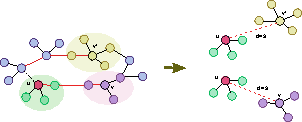
\includegraphics[width=.9\textwidth]{img/cdnk}
\caption{Pairwise neighborhood subgraphs for the ``red'' node with $r=1$ and $d=3$ using ``conjuction'' and ``disjuctive'' edges}
\label{fig:cdnk}
\end{figure}

\subsection{Real valued node information}
In order to integrate the information of real vectors we proceed as follows. We compute a sparse vector representation for the neighborhood graph rooted in node $v$ following \cite{costa2010fast}: for each neighborhood subgraph we calculate the quasi-isomorphism certificate hash code; we then combine the hashes for the pair of neighborhoods and use the resulting integer as a feature indicator. This yields a direct sparse vector representation (associated to node $u$ in graph $G$) $f: G_u \longmapsto I\!R^L$ where $L \approx 10K-1M$. Given the real valued vector information (associated to node $u$ in graph $G$) $g: G_u \longmapsto I\!R^K$ computed as the multi-class similarity to the $K$ clusters (c.f.r. Section \ref{sec:lab}), we update the computation of CDNK considering the discrete convolution of the discrete information with the real valued information:   
\begin{equation}
K(G_u,G_{u'}) = \left< f(G_u) \bigotimes g(G_u), f(G_{u'}) \bigotimes g(G_{u'}) \right>
\end{equation}
where the discrete convolution is defined as: 
$(f \bigotimes g)[n]=\sum _{m=0}^{K-1}f[n-m]g[m].$
In words, we are starting a scaled copy of the real valued vector at the position indicated by each feature computed on the basis of the discrete information. Intuitively, when both the real valued and the discrete information match, the kernel computes a large similarity, but if there is a discrepancy in either one of the sources of information, the similarity will be penalized. 


\subsection{Network Decomposition} 
In gene-disease associations networks it is not uncommon to find nodes with high degrees. Unfortunately these cases cannot be effectively processed by a neighborhood based decomposition kernel (see \ref{sec:k}) since these are based on the notion of exact matches and the probability of finding identical neighborhoods decreases exponentially as the degree increases. This means that in a finite network it quickly becomes impossible to find any match and hence learn or generalize at all. As an alternative, we propose a procedure to ``sparsify'' the network that is observed by the neighborhood kernel. In reality we do not alter the cardinality of the edge set, but rather mark the edges with special attributes that will inform the kernel computation. The result is a procedure that decomposes the network in a linked collection of sparse sub-networks where each node has a reduced connectivity when considering the edges of a specific type. However the other edges are still available to connect the various sub-networks. We distinguish two types of edges: {\em conjunctive} and {\em disjunctive} edges. Nodes linked by conjunctive edges are going to be used jointly to define the notion of context and will be visible to the neighborhood graph kernel. Nodes linked by disjunctive edges are instead used to define features based only on the pairwise co-occurrence of the genes at the endpoints and are processed by our novel kernel.




\textit{Iterative k-core decomposition} \cite{alvarez2005k}: The node set is partitioned in two groups on the basis of the degree of each node w.r.t. a threshold degree $D$, the first part contains all nodes with degree smaller or equal than $D$ and the second part the remaining ones. The node partition is used to induce the ``conjunctive'' vs ``disjunctive'' notion for the edge partition: edges that have both endpoints in the same part are marked as conjunctive, otherwise they are marked as disjunctive. We apply the k-core decomposition iteratively, where at each iteration we consider only the graph induced by the conjunctive edges. We stop iterating the decomposition after a user defined number of steps. Note that this decomposition does not alter the cardinality of the edge set, it is simply a procedure to mark each edge with the attribute conjunctive or disjunctive.  

\begin{figure}
\centering
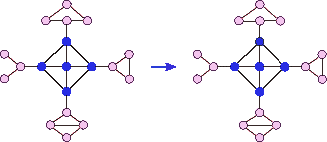
\includegraphics[width=.9\textwidth]{img/k_core}
\caption{K-core decomposition with degree threshold $D = 5$}
\label{fig:example}
\end{figure}

\textit{Clique decomposition} \cite{tarjan1985decomposition}: To model the notion that nodes in a clique are tightly related, we summarize the whole clique with a new ``representative'' node. All the cliques (completely connected subgraphs) with a number of nodes greater than or equal a threshold size $C$ are identified. The endpoints of all edges incident on the clique's nodes are moved to the representative node. Disjunctive edges are introduced to connect each node in the clique to the representative. Finally all edges with both endpoints in the clique are removed.

In our work a network is transformed by applying first the iterative k-core decomposition and then the clique decomposition.

\begin{figure}
\centering
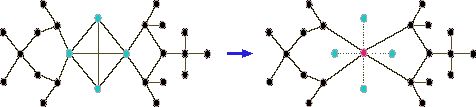
\includegraphics[width=.9\textwidth]{img/clique}
\caption{Clique decomposition with threshold $C = 4$}
\label{fig:example}
\end{figure}

\section{Experiments}
We perform an empirical evaluation of the predictive performance of several kernel based methods on two of the databases used in \cite{chen2014disease}.

\textbf{BioGPS:} A gene co-expression network is constructed from BioGPS dataset, which contains 79 tissues, measured with the Affymetrix U133A array. Edges are inserted when the pairwise Pearson correlation coefficient (PCC) between genes is larger than 0.5.

\textbf{Pathways:} Pathway information is retrieved from KEGG, Reactome, PharmGKB and the Pathway Interaction Database. If a couple of proteins co-participate in any pathway, the two corresponding genes are linked.  

To compare the performance of graph node kernels we focus on the {\em gene prioritization} problem, which is the task to rank genes based on their probabilities to be related to a specific disease given a set of genes known to be associated to the disease. We follow \cite{chen2014disease} and analyze  12 diseases \cite{goh2007human} for which it is known that at least 30 genes are involved. For each disease, we construct a positive set $\mathcal{P}$ with all confirmed disease genes, and a negative set $\mathcal{N}$ which contains random genes associated at least to one disease class which is not related to the class that is defining the positive set. In \cite{chen2014disease} the ratio between the dataset sizes is chosen as $\vert \mathcal{N} \vert = \frac{1}{2} \vert \mathcal{P} \vert$. The predictive performance of each method is evaluated via a leave-one-out cross validation: one gene is kept out in turn and the rest are used to train an SVM model. We compute a decision score $q_i$ for the test gene $g_i$ as the top percentage value of score $s_i$ among all candidate gene scores. We collect all decision scores for every gene in the training set to form a global decision score list on which we compute the AUC-ROC.

\textbf{Model Selection:}
The hyper parameters of the various methods are tuned using a k-fold strategy. However due to the non i.i.d. nature of the problem, we employ a stronger setup to ensure no information leakage. The dataset on which we are validating the performance is never subsequently used in the predictive performance estimate. The values for diffusion parameter in DK and MED are sampled in $\lbrace 10^{-3}, 10^{-3}, 10^{-2}, 10^{-1} \rbrace$, time steps in MD in $\lbrace 1, 10, 100 \rbrace$ and RL parameter in $\lbrace 1, 4, 7 \rbrace$. For CDNK, the degree threshold values are sampled in $\lbrace 10,\ 15,\ 20 \rbrace$, clique size threshold in $\lbrace 4,\ 5 \rbrace$, maximum radius in $\lbrace 1,\ 2 \rbrace$, maximum distance in $\lbrace 2,\ 3,\ 4 \rbrace$, nuber of clusters $K$ in $\lbrace 5,\ 7 \rbrace$. Finally, the regularization trade off parameter $C$ for the SVM is sampled in $\lbrace 10^{-5},  \ 10^{-4}, \ 10^{-3},\ 10^{-2},\ 10^{-1}, 1,\ 10,\ 10^2 \rbrace$.

\section{Results and discussion}
Table \ref{table_biogps} and \ref{table_pathways} show the AUC performance of different graph node kernel models. Predictive models based on CDNK variations are ranked in top positions in all cases on BioGPS dataset and 9 out of 11 cases on Pathways when compared to diffusion based kernels. CDNK is ranking first when considering both the average AUC-ROC and the average rank with a difference, w.r.t. the best diffusion kernel, ranging from 5.4$\%$ to 10$\%$ and from 1.2$\%$ to 3.2$\%$ on BioGPS and Pathways, respectively. Regarding the variations of CDNK, the integration of real valued vector information improves the performance in most cases on using discrete labels only. The improvement in average ranges from 1.3$\%$ to 4.6$\%$. Note that also in the case where only topological information is used to induce the discrete label (CDNK3 in the Table \ref{table_biogps} and \ref{table_pathways}), the proposed approach improves on state-of-the-art. 

%It is worth noticing that on average the rank of CDNK with real vector information are high in both ways of discrete labeling and on both databases.

%Table \ref{table_biogps} and \ref{table_pathways} show the AUC performance of the models trained by using different graph node kernels on 11 gene-disease association problems using the BioGPS and Pathways datasets to materialize the gene relation network. We note that CDNK ranks first in 7 out of 11 cases using  both networks. CDNK is the top performant kernel also when considering the average AUC ROC and the average rank with 73.3/2.0, 76.5/1.8, with a difference w.r.t. the second best of 5.5$\%$ and 1$\%$ on BioGPS and Pathways, respectively. MED and RL show similar and moderate results with small gap between them. DK and MD exhibit modest performance on average and  are ranked last in many cases: 7 times out of 11 for MD in BioGPS and 10 out of 11 for DK in Pathways. Low performance cases include networks that have high {\em average} node degree which is likely to yield very sparse and fragmented network decompositions.
%======================================================
\begin{table}
\caption{\textit {Predictive performance on 11 gene-disease associations in percentage using network induced by the BioGPS. Best results in bold. We report the AUC ROC and the rank for each kernel method.  CDNK1 = ontology for discrete labels, CDNK2 = ontology for both discrete and vector labels, CDNK3 = node degree for discrete labels and CDNK4 = node degree for discrete labels and ontology for vector label.}}
\vspace*{5pt}
\centering
\setlength{\tabcolsep}{1mm}
\begin{tabular}{|c|c|c|c|c|c|c|c|c|}
\hline
         & \multicolumn{8}{c|}{\textbf{BioGPS}}\\
 \hline
Disease & DK & MD & MED & RL & CDNK1 & CDNK2 & CDNK3 & CDNK4\\

 \hline
1 & 51.9/8 & 57.4/7 & 59.0/6 & 59.2/5 & 65.1/4 & 69.5/2 & 69.3/3 & \textbf{70.3/1} \\
2 & 81.7/5 & 78.5/6 & 75.2/7 & 75.0/8 & 88.3/2 & \textbf{88.8/1} & 85.1/4 & 86.8/3 \\
3 & 64.3/7 & 59.6/8 & 71.6/3 & 71.8/2 & 65.5/5 & \textbf{72.5/1} & 64.7/6 & 66.4/4 \\
4 & 65.3/7 & 58.2/8 & 67.8/6 & 67.8/5 & 71.9/4 & \textbf{78.7/1} & 73.9/3 & 77.0/2 \\
5 & 64.0/8 & 64.1/7 & 66.5/5 & 66.2/6 & 75.9/4 & 76.2/3 & 76.9/2 & \textbf{77.4/1} \\
6 & 74.6/5 & 70.2/8 & 71.0/7 & 71.2/6 & 79.3/2 & \textbf{83.7/1} & 76.7/4 & 79.0/3 \\
7 & 73.0/5 & 66.7/8 & 75.4/3 & 75.6/2 & 68.8/6 & 73.9/4 & 67.3/7 & \textbf{76.9/1} \\
8 & 74.4/8 & 76.8/3 & 76.2/5 & 76.4/4 & 74.7/7 & \textbf{77.7/1} & 76.0/6 & 76.8/2 \\
9 & 71.5/2 & 65.6/8 & 67.7/5 & 69.9/3 & 66.8/7 & \textbf{71.7/1} & 67.1/6 & 68.1/4 \\
10 & 54.0/6 & 50.3/8 & 56.1/5 & 51.1/7 & 77.6/4 & \textbf{82.7/1} & 80.5/2 & 80.0/3 \\
11 & 58.2/7 & 51.3/8 & 59.3/6 & 59.3/5 & 71.8/4 & \textbf{80.2/1} & 75.3/3 & 77.1/2 \\
\hline
$\overline{AUC}$ & 66.6 & 63.5 & 67.8 & 67.6 & 73.2 & \textbf{77.8} & 73.9 & 76.0 \\
$\overline{Rank}$ & 	6.18 & 7.18 & 5.27 & 4.82 & 4.45 & \textbf{1.55} & 4.18 & 2.36 \\
 \hline 
\end{tabular}
\label{table_biogps}
\end{table}
%==================================================
\begin{table}
\caption{\textit {Predictive performance on 11 gene-disease associations in percentage using network induced by the Pathways. Best results in bold. We report the AUC ROC and the rank for each kernel method.  CDNK1 = ontology for discrete labels, CDNK2 = ontology for both discrete and vector labels, CDNK3 = node degree for discrete labels and CDNK4 = node degree for discrete labels and ontology for vector label.}}
\vspace*{5pt}
\centering
\setlength{\tabcolsep}{1mm}
\begin{tabular}{|c|c|c|c|c|c|c|c|c|}
\hline
         & \multicolumn{8}{c|}{\textbf{Pathways}} \\
 \hline
Disease & DK & MD & MED & RL & CDNK1 & CDNK2 & CDNK3 & CDNK4 \\

 \hline
1 & 74.7/8 & 76.4/7 & 78.7/6 & 78.8/5 & 80.2/3 & \textbf{82.4/1} & 80.6/2 & 79.4/4 \\
2 & 55.1/8 & 64.9/7 & 76.6/6 & 76.6/5 & 81.1/2 & 80.3/3 & 79.8/4 & \textbf{82.2/1} \\
3 & 55.0/8 & 62.7/7 & 64.1/5 & 65.6/4 & 67.1/3 & 63.6/6 & 68.5/2 & \textbf{71.5/1} \\
4 & 54.3/8 & 65.2/7 & \textbf{73.7/1} & 73.7/2 & 66.1/5 & 68.1/3 & 67.5/4 & 65.6/6 \\
5 & 52.9/8 & 55.7/7 & 62.7/5 & 62.7/6 & 68.3/2 & \textbf{69.6/1} & 66.3/4 & 66.8/3 \\
6 & 83.4/8 & 92.7/7 & 96.5/2 & \textbf{96.5/1} & 93.0/6 & 94.1/5 & 94.4/4 & 95.5/3 \\
7 & 84.5/8 & 88.3/7 & 89.4/3 & 89.5/2 & 88.5/6 & 88.5/5 & 88.7/4 & \textbf{90.5/1} \\
8 & 53.7/8 & 65.6/7 & 72.0/6 & 72.3/5 & 72.5/3 & 72.5/2 & 72.3/4 & \textbf{76.5/1} \\
9 & 52.5/8 & 64.9/5 & 64.2/7 & 64.2/6 & \textbf{81.3/1} & 81.0/2 & 79.6/3 & 78.8/4 \\
10 & 68.8/6 & 65.4/8 & 74.4/5 & 74.4/4 & 66.9/7 & 76.8/2 & 76.1/3 & \textbf{79.5/1} \\
11 & 53.7/8 & 69.2/7 & 74.6/5 & 74.1/6 & 77.0/2 & \textbf{78.7/1} & 75.4/4 & 77.0/3 \\
\hline
$\overline{AUC}$ & 62.6 & 70.1 & 75.2 & 75.3 & 76.5 & 77.8 & 77.2 & \textbf{78.5} \\
$\overline{Rank}$ & 7.82 & 6.91 & 4.64 & 4.18 & 3.64 & 2.82 & 3.45 & \textbf{2.55} \\
 \hline 
\end{tabular}
\label{table_pathways}
\end{table}

\section{Conclusion}
We have shown how decomposing a network in a set of connected sparse graphs allows us to take advantage of the discriminative power of CDNK, a novel decomposition kernel, to achieve state-of-the-art results. Moreover, we have also introduced the way to integrate ``side'' information in form of real valued vectors when it is available on graph to get even better performance of CDNK. In future work we will investigate how to \textit{i}) decompose networks in a data driven way and \textit{ii}) extend the CDNK approach to gene-disease association problems exploiting multiple heterogeneous information sources in a joint way.
\chapter{Joint Neighborhood Subgraphs for Link Prediction}
\label{chap:jnsl}
\section{Motivation}
We are witnessing a constant increase of the rate at which data is being produced and made available in machine readable formats. Interestingly it is not only the quantity of data that is increasing, but also its complexity, i.e. not only are we measuring a number of attributes or features for each data point, but we are also capturing their mutual relationships, that is, we are considering non independent and identically distributed (non i.i.d.) data. This yields collections that are best represented as graphs or relational data bases and requires a more complex form of analysis. As cursory examples of application domains that are social networks, where nodes are people and edges encode a type of association such as friendship or co-authorship, bioinformatics, where nodes are proteins and metabolites and edges represent a type of chemical interaction such as catalysis or signaling, and e-commerce, where nodes are people and goods and edges encode a ``buy'' or ``like'' relationship.
A key characteristic of this type of data collections is the sparseness and dynamic nature, i.e. the fact that the number of recorded relations is significantly smaller than the number of all possible pairwise relations, and the fact that these relations evolve in time. A crucial computational task is then the ``link prediction problem'' which allows to suggest friends, or possible collaborators for scientists in social networks, or to discover unknown interactions between proteins to explain the mechanism of a disease in biological networks, or to suggest novel products to be bought to a customer in a e-commerce recommendation system. Many approaches to link prediction that exist in literature can be partitioned according to \textit{i}) whether additional or ``side'' information is available for nodes and edges or rather only the network topology is considered and \textit{ii}) whether the approach is unsupervised or supervised. 

Unsupervised methods are non-adaptive (i.e. they do not have parameters that are tuned on the specific problem instance), and can therefore be computationally efficient. In general they define a score for any node pair that is proportional to the existence likelihood of an edge between the two nodes. \textit{Adamic-Adar} \cite{adamic} computes the weighted sum over the common neighbors where the weight is inversely proportional to the (log of) each neighbor node degree. The \textit{preferential attachment} method computes a score simply as the product of the node degrees in an attempt to exploit the ``rich get richer'' property of certain network dynamics. \textit{Katz} \cite{katz} takes into account the number of common paths with different lengths between two nodes, assigning more weight to shorter paths. The \textit{Leicht-Holme-Newman} method \cite{lhni} computes the number of intermediate nodes. In \cite{matrix-factorization} the score is derived from the singular value decomposition of the adjacency matrix. 

Supervised link prediction methods convert the problem into a binary classification task where links present in the network (at a given time) are considered as positive instances and a subset of all the non links are considered as negative instances. Following \cite{matrix-factorization}, we can further group these methods into four classes: feature-based models, graph regularization models, latent class models and latent feature models. 
A Bayesian nonparametric approach is used in \cite{nonparametric} to compute a nonparametric latent feature model that does not need a user defined number of latent features but rather induces it as part of the training phase. 
In \cite{matrix-factorization} a matrix factorization approach is used to extract latent features that can take into consideration the output of an arbitrary unsupervised method. The authors show a significant increase in predictive performance when considering a ranking loss function suitable for  the imbalance problem, i.e. when the number of negative is much larger than the number of positive instances. 

In general supervised methods exhibit better accuracies compared to unsupervised methods although incurring in much higher computational and memory complexity costs.
Moreover, most approaches implicitly represent the link prediction problem and the inference used to tackle it as a disjunction over the edges, that is, information on edges is propagated in such a fashion so that for a node to have $k$ neighbors or $k+1$ does not make a drastic difference.
We claim that this hypothesis is likely putting a cap on the discriminative power of classifiers and therefore we propose a novel supervised method that employs a conjunctive representation. We call the method ``joint neighborhood subgraphs link prediction'' (JNSL). The key idea here is to transform the link prediction task into a binary classification on suitable small subgraphs which we then solve using an efficient graph kernel method.
\section{Method}
\subsection{Definitions and notation}
We represent a problem instance as a graph $G=(V,E)$ where $V$ is the set of nodes and $E$ is the set of links. The set $E$ is partitioned into the subset of observed links ($O$) and the subset of unobserved links ($U$). Like other approaches we assume that all un-observed links are indeed ``non-links'' and we therefore define the link prediction problem as the task of ranking candidate links from the most to the least probable to recover links in $O$ but not in $U$ exploiting only the network topology.


We define the \textit{distance} $\mathcal{D}(u,v)$ between two nodes $u$ and $v$, as the number of edges on the shortest path between them. The \textit{neighborhood} of a node $u$ with radius $r$, $N_r(u) = \lbrace v\ |\ \mathcal{D}(u,v) \leq r \rbrace$, is the set of nodes at distance no greater than $r$ from $u$. The corresponding \textit{neighborhood subgraph} $\mathcal{N}_{r}^{u}$ is the  subgraph induced by the neighborhood (i.e. considering all the edges with endpoints in $N_r(u)$). The \textit{degree} of a node $u$, $d(u) = |\mathcal{N}_{1}^{u}|$, is the cardinality of its neighborhood. The maximum node degree in the graph $G$ is $d(G)$.

\subsection{Link encoding as subgraphs union}
\label{sec:link}
Most methods for link prediction compute pairwise nodes similarities treating  the nodes defining the candidate edge independently. Instead we propose to jointly consider both candidate endpoint nodes together with their extended ``context''. To do so we build a graph starting from the two nodes and the underlying network. Given nodes $u$ and $v$, we first extract the two neighborhood sets with a user defined radius $R$ rooted at $u$ and $v$ to obtain $N_R(u)$ and $N_R(v)$, respectively. We then consider the graph $\mathcal{J}$ induced by the set union $N_R(u) \cup N_R(u)$. Finally we add an auxiliary node $w$ and the necessary edges to connect it to $u$ and $v$ (see Fig.\ref{fig:example}).

\begin{figure}
\centering
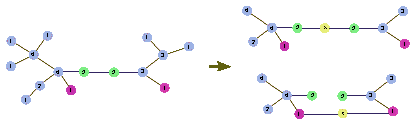
\includegraphics[width=.9\textwidth]{img/subgraphs.pdf}
\caption{Left) We represent with solid lines edges belonging to the training material and with a dotted line edges belonging to the test material. Right) joint neighborhood subgraphs for an existing (green endpoints) (top) and a non existing (red endpoints) link (bottom). These graphs will receive respectively a positive and a negative target.}
\label{fig:example}
\end{figure}

\subsection{Node labeling}
We propose to use a graph kernel approach to classify the subgraphs encoding each link. In our setup nodes are not endowed with any ``side'' information. However to increase the discriminative power of the similarity notion induced by the graph kernel, instead of assuming a dummy, non-informative label on each node, we propose to use a node labeling function $\ell$ which assigns as the discrete label the node degree. More precisely, for nodes having degree less than or equal than a user defined threshold $T$ ($T=5$ in our experimental evaluation) we use as label the degree value. Degree values larger than $T$ are subsequently discretized into $k$ levels. Here the implicit assumption is that nodes with similar degrees have common properties. Formally, the labeling function is defined as:
\begin{center}
$\ell(u) = \left\{
	\begin{array}{ll}
		d(u),\  & \mbox{if } d(u) \leq T \\
		T+i,\ & \mbox{if } d(u) > T
	\end{array}
\right.$,
\end{center}
where $i = \lceil \frac{d(u)-T}{bin}\rceil$, $bin = \frac{d(G)-T}{\lambda - T}$ and $\lambda$ ($\lambda > T$) is the maximum number of symbols used. The value of $\lambda$ depends on the degree distribution and can be tuned as a hyperparameter of the approach.

\subsection{The graph kernel}
Here we briefly describe an efficient graph kernel called the Neighborhood Subgraph Pairs Distance kernel (NSPDK) introduced in \cite{nspdk}. NSPDK is an instance of ``decompositional'' kernels \cite{convolution-kernel} based on the idea of counting the number of common small subgraphs between two graphs. The subgraphs are pairs of neighborhoods whose roots are at a short distance. 

Given a labeled graph $G \in \mathcal{G}$ and two rooted graphs $A_u, B_v$, we first define the relation $R_{r,d}(A_u, B_v, G)$ to be true {\em iff} $A_u \cong \mathcal{N}_r^u$ is (up to isomorphism $\cong$) a neighborhood subgraph with radius $r$ of $G$ and so is $B_v \cong  \mathcal{N}_r^v$, such that $v$ is a distance $d$ from $u$: $\mathcal{D}(u,v)= d$. We then define the inverse relation $R^{-1}$ that returns all pairs of neighborhoods of radius $r$ at distance $d$ in $G$, $R^{-1}_{r,d}(G) = \lbrace A_u, B_v | R_{r,d}(A_u,B_v,G)=true\rbrace$. The kernel $\kappa_{r,d}$ over $\mathcal{G} \times \mathcal{G}$ is the number of such fragments in common in two input graphs:
\begin{center}
$\kappa_{r,d}(G,G^{'}) = 
\!\!\!\!\!\!\!\!\!\!\!\! 
\sum\limits_{\substack{A_u, B_v \ \in \ R_{r,d}^{-1}(G) \\ 
{A'}_{u'}, {B'}_{v'} \ \in \ R_{r,d}^{-1}(G')
}} \!\!\!\!\!\!\!\!\!\!\!\!  { { \textbf{1}_{A_{u} \cong A'_{u'}}} \cdot {
\textbf{1}_{B_{v} \cong B'_{v'}}} }$, 
\end{center}
\noindent where $\textbf{1}_{A \cong B}$ is the \textit{exact matching function} that returns 1 if $A$ is isomorphic to $B$ and 0 otherwise. Finally, the NSPDK is defined as $K(G,G') = \sum\limits_{r}{\sum\limits_{d}{\kappa_{r,d}(G,G')}}$, where for efficiency reasons, the values of $r$ and $d$ are upper bounded to a given maximal $r^*$ and $d^*$, respectively.

% Related to exact matching function, this function needs to solve the graph isomorphism problem. This problem is not known to be solvable in polynomial time nor to be NP-complete. In \cite{nspdk}, they propose an approximate method to figure out graph isomorphism problem. It first transforms graphs into strings. It then employ a hash function to map each unique string with an integer number. Finally, two graphs are isomorphic if they have the same corresponding integer numbers.

\subsection{Joint neighborhood subgraphs link prediction}
In the link prediction problem we are given a graph $G(V,E)$ and a binary target vector $Y=\{y_{(0,0)},y_{(0,1)}, \cdots, y_{(|V|,|V|)}\}$ where $y_{(u,v)}=1$ if $(u,v) \in E$ and 0 otherwise. The training data is obtained considering a random subset of edges in $E^{tr} \in E$ and inducing a training graph $G^{tr}=(V,E^{tr})$. Note that the graph used for training does not contain any of the edges that will be queried in the test phase. The remaining edges $E^{ts} = E \setminus E^{tr}$ are used to partition the target vectors: $Y^{tr} = \{y_{(u,v)} | (u,v) \in E^{tr}\}$, $Y^{ts} = \{y_{(u,v)} | (u,v) \in E^{ts}\}$.
We can now cast the problem as a standard classification problem in the domain of graphs. Given $G^{tr}$ we build a train and test set as the corresponding joint neighborhood subgraphs as detailed in Section~\ref{sec:link}. 
We can now compute a Gram matrix of the instances and solve the classification task using for example the efficient LinearSVC library \cite{svm}.
\section{Experiments}
\section{Empirical evaluation}
To compare the performance of the JNSL method with other link prediction approaches we follow \cite{matrix-factorization} and use 6 datasets belonging to different domains.
\begin{itemize}
\item \textit{Protein }\cite{protein-protein}: nodes are proteins and edges encodes a thresholded interaction confidence between proteins. It has 2617 nodes and 11855 links with an average degree of 9.1.

\item \textit{Metabolic} \cite{metabolic}: nodes are enzyme and metabolites, edges are present if the enzyme catalyzes for a reaction that include those chemical compounds. It has 668 nodes and 2782 links with an average degree of 8.3.

\item \textit{Nips} \cite{nips}: nodes are authors at the NIPS conference from the first to the $12^{th}$ edition. Links encode the co-authorhip relation, i.e. if two authors have published a paper together. This network contains 2865 nodes and 4733 links with an average degree of 3.3.

\item \textit{Condmat} \cite{condmat}: nodes are scientists working in condensed matter physics, edges encode co-authorship. This network has 14230 nodes and 1196 links with an average degree of 0.17.

\item \textit{Conflict} \cite{conflict1}, \cite{conflict2}: nodes are countries and edges encode a conflict or a dispute. We have 130 nodes and 180 links in total in this network with an average degree of 2.5.

\item \textit{Powergrid} cite{powergrid}: a network of electric powergrid in US. It has 4941 nodes and 6594 links. The average degree is 2.7.
\end{itemize}

We evaluate the performance of employed methods by splitting 10 times the data in a train and a test part. For \textit{Protein}, \textit{Metabolic}, \textit{Nips} and \textit{Conflict} networks, we use 10$\%$ of the edges to induce the training set while for \textit{Condmat} and \textit{Powergrid} we use 90$\%$ of the links. The performance of each method is computed as the average of the AUC-ROC over the 10 rounds.

\textbf{Model Selection}: The values of different hyper-parameters are set by using a 3-fold on the training set, that is, always considering only the training network, we use one fold for fitting the parameters and the rest two folds for validating the effect of the hyper parameter choice. We tune the values of radius for extracting subgraphs $R$ in $\lbrace 1, 2 \rbrace$, $\lambda$ in node label function in $\lbrace 10, 15 \rbrace$, for $r$ and $d$ parameters of NSPDK in $\lbrace  1, 2 \rbrace$ and $\lbrace  1, 2, 3 \rbrace$, respectively. Finally, the regularization tradeoff $C$ for the SVM is picked up in $\lbrace 10^{-4}, 10^{-3}, 10^{-2},\ 10^{-1}, 1,\ 10,\ 10^2, 10^3,\ 10^4 \rbrace$.
\section{Results and discussion}
In Table \ref{result_table}, we report the performance of link prediction methods measured as the AUC-ROC value on 6 datasets. From the results on the table, we can group methods into two groups based on their performances: supervised methods and unsupervised methods. The performance of supervised methods are considerably higher than unsuperivsed ones in most cases, except in the Conflict dataset where Sup-Top outperforms Fact+Scores, but with a very small difference. Concerning supervised methods, JNSL outperforms Fact-Scores in all cases. The difference between their performance is small in PowerGrid and Protein datasets with 0.5$\%$ and 0.8$\%$, respectively. And the big gap is in the Condmat dataset with 7.4$\%$. 
\begin{table}[t!]
\caption{AUC-ROC performance on 6 datasets. Legend: AA: Adamic-Adar, PA \cite{pa} preferential Attachment, SHP: Shortest Path, Sup-Top \cite{matrix-factorization}: Liear regression running on unsupervised scores, SVD \cite{matrix-factorization}: Singular value decomposition, Fact+Scores \cite{matrix-factorization}: Factorization with unsupervised scores, JNSL: joint neighborhood subgraph link (our method). In bold the highest score.}
\centering
\setlength{\tabcolsep}{1mm}
\begin{tabular}{|c|c|c|c|c|c|c|}
\hline
         & \multicolumn{6}{c|}{\textbf{Datasets}}\\
 \hline
\textbf{Methods} & Protein & Metabolic & Nips & Condmat & Conflict & PowerGrid\\
	& ($\%$) & ($\%$) & ($\%$) & ($\%$) & ($\%$) & ($\%$)\\
\hline
AA & 56.4$\pm$0.5 & 52.4$\pm$0.5 & 51.2$\pm$0.2 & 56.7$\pm$1.4 & 50.7$\pm$0.8 & 58.9$\pm$0.3\\
PA & 75.0$\pm$0.3 & 52.4$\pm$0.5 & 54.3$\pm$0.5 & 71.6$\pm$2.6 & 54.6$\pm$2.4 & 44.2$\pm$01.0\\
SHP & 72.6$\pm$0.5 & 62.6$\pm$0.4 & 51.7$\pm$0.3 & 67.3$\pm$1.8 & 51.2$\pm$1.4 & 65.9$\pm$1.5\\
Katz & 72.7$\pm$0.5 & 60.8$\pm$0.7 & 51.7$\pm$0.3 & 67.3$\pm$1.7 & 51.2$\pm$1.4 & 65.5$\pm$1.6 \\
Sup-Top & 75.4$\pm$0.3 & 62.8$\pm$0.1 & 54.2$\pm$0.7 & 72.0$\pm$2.0 & 69.5$\pm$7.6 & 70.8$\pm$6.2\\
SVD & 63.5$\pm$0.3 & 53.8$\pm$1.7 & 51.2$\pm$3.1 & 62.9$\pm$5.1 & 54.1$\pm$9.4 & 69.1$\pm$2.6\\
Fact+Scores & 79.3$\pm$0.5 & 69.6$\pm$0.2 & 61.3$\pm$1.9 & 81.2$\pm$2.0 & 68.9$\pm$4.2 & 75.1$\pm$2.0 \\
JNSL & \textbf{80.1$\pm$0.8} & \textbf{72.5$\pm$0.7} & \textbf{62.1$\pm$0.8} & \textbf{88.6$\pm$2.3} & \textbf{72.0$\pm$0.9} & \textbf{75.6$\pm$0.7} \\
 \hline 
\end{tabular}
\label{result_table}
\end{table}

\section{Conclusion}
We have presented a novel approach to link prediction in absence of side information that can effectively exploit the topological contextual information available in the neighborhood of each edge. We have empirically shown that this approach achieves very competitive results compared to other state-of-the-art methods.
In future work, we will investigate how to make use of multiple and heterogeneous information sources when these are available for nodes and edges.
\chapter{Link Enrichment for Diffusion-based Graph Node Kernel}
\section{Motivation}
\section{Method}
\section{Experiments}
\section{Analysis}
\section{Conclusion}
\chapter{Scuba - Scalable Kernel-based Gene Prioritization}
\label{chap:scuba}
\section{Motivation}
The identification of the genes underlying human diseases is a major goal in current molecular genetics research. Dramatic progresses have been made since the 1980s, when only a few DNA loci were known to be related to disease phenotypes. Nowadays opportunities for the diagnosis and the design of new therapies are progressively growing, thanks to several technological advances and the application of statistical or mathematical techniques. For instance, positional cloning has allowed to map a vast portion of known Mendelian diseases to their causative genes \cite{strachan,botstein}. However, despite the huge advances, much remains to be discovered. On December 21\textsuperscript{st} 2016, the Online Mendelian Inheritance in Man database (OMIM) registered 4,908 Mendelian phenotypes of known molecular basis and 1,483 Mendelian phenotypes of unknown molecular origin \cite{omim}. Moreover, 1,677 more phenotypes were suspected to be Mendelian. But it is among oligogenic and poligenic (and multifactorial) pathologies that the most remains to be elucidated: for the majority of them, only a few genetic loci are known \cite{strachan,botstein}.

Independently of the type of disease, the search of causative genes usually concerns a large number of suspects. It is therefore necessary to recognise the most promising candidates to submit to additional investigations, as experimental procedures are often expensive and time consuming. Gene prioritization is the task of ordering genes from the most promising to the least. In traditional genotype-phenotype mapping approaches - as well as in genome-wide association studies - the first step is the identification of the genomic region(s) wherein the genes of interest lie. Once the candidate region is identified, the genes there residing are prioritized and finally analysed for the presence of possible causative mutations \cite{strachan}. More recently, in new generation sequencing studies this process is inverted as the first step is the identification of mutations, followed by prioritization and final validation \cite{salgado}. Prioritization criteria are usually based on functional relationships, co-expression and other clues linking genes together. In general, all of them follow the ``guilt-by-association" principle, i.e. disease genes are sought by looking for similarities to genes already associated to the pathology of interest \cite{strachan}.

In the last few years, computational techniques have been developed to aid researchers in this task, applying both statistics and machine learning \cite{moreau}. Thanks to the advent of high-throughput technologies and new generation sequencing, a huge amount of data is in fact available for this kind of investigations. In particular, computational methods are essential for multi-\emph{omics} data integration, that has been recognised as a valuable strategy for understanding genotype-phenotype relationships \cite{ritchie}. In fact, clues are often embedded in different data sources and only their combination leads to the emergence of informative patterns. Furthermore, incompleteness and noise of the single sources can be overcome by inference across multiple levels of knowledge.

Several popular algorithms for pattern analysis are based on \emph{kernels}, which are mathematical transformations that permit to estimate the similarity among items (in our case genes) taking into account complex data relations \cite{cristianini}. Importantly, kernels provide a universal encoding for any kind of knowledge representation, e.g. vectors, trees or graphs. When data integration is required, a multiple kernel learning (MKL) strategy allows a data-driven weighting/selection of meaningful information \cite{gonen}. The goal of MKL is indeed to learn optimal kernel combinations starting from a set of predefined kernels obtained by various data sources. Through MKL the issue of combining different data types is then solved by converting each dataset in a kernel matrix.

Numerous MKL approaches have been proposed for the integration of genomic data \cite{wang,borgwardt} and some of them have been applied to gene prioritization \cite{debie,mkl1class,prodige,zakeri}. De Bie \emph{et al} formulated the problem as a one-class support vector machine (SVM) optimization task \cite{debie}, while Mordelet and Vert tackled it through a biased SVM in a \emph{positive-unlabelled} framework \cite{prodige,chapelle}. Recently, Zakeri \emph{et al} proposed an approach for learning non-linear log-euclidean kernel combinations, showing that it can more effectively detect complementary biological information compared to linear combinations-based approaches \cite{zakeri}. However, as highlighted in a recent work by Wang \emph{et al} \cite{wang}, current methods share two limitations: high computational costs - given by a (at least) quadratic complexity in the number of training examples - and the difficulty to predefine optimal kernel functions to be fed to the MKL machine.

In this work we tackle these issues by proposing a novel scalable gene prioritization method based on a particular MKL approach \cite{easymkl}. By this approach, the optimal kernel is efficiently computed by maximizing the distance between positive and negative examples and optimizing the margin distribution \cite{komd}. This permits to obtain a high scalability relatively to the number of kernels, with a linear time complexity and a practically constant memory requirement. However, this approach assumes comparable label noise in the two example distributions, which does not reflect the case in consideration. Moreover, it does not scale with the number of training examples. Here we introduce a new algorithm, specifically adapted to a \emph{positive-unlabelled} unbalanced framework and we apply it to gene prioritization for the first time. The new learning algorithm has an additional gain in scalability that comes particularly useful when large numbers of genes have to be prioritized. This scalability allows us to transform each data source by multiple kernels and alleviates the issue of defining appropriate base kernels for each source. We called the proposed method Scuba (SCalable UnBAlanced gene prioritization).

From an experimental point of view, here we focus on the integration of multiple gene networks whose edges symbolize functional relationships from heterogeneous sources and we employ two different test settings. In the first setting, we reproduce the procedure presented in a previous work by Chen \emph{et al} \cite{f3pc}, built upon cross-validation experiments \cite{devijver} on collections of known disease genes. This kind of evaluation is useful to compare different methods, but results may suffer from overestimation due to the reliance of many data repositories on medical literature or external data sources like OMIM \cite{omim}. Such dependence introduces a bias that may favour the retrieval of known disease genes. Thus, as a second validation we employ a more realistic setting, following a previous evaluation of gene prioritization tools by B\"ornigen \emph{et al} \cite{bornigen}. Here performance measures focus on the ability of predicting disease genes discovered subsequently to the last update of datasets.

\textcolor{red}{Overall, we compare Scuba with other 14 gene prioritization systems, including other 2 kernel-based methods and 8 web tools}. We find that Scuba has competitive accuracy and in particular yields the best results in genome-wide prioritizations, showing its value for large-extent applications.
\section{Method}
In this section, we first introduce and formalize some concepts that will be used throughout this paper. Then, we present the proposed approach in detail.

\textbf{Disease gene prioritization}: Let us consider a set of genes $\mathcal{G} = \lbrace g_1, g_2, \ldots, g_N \rbrace$ that represents either the global set of genes in the genome or a subset of it. Given another set $\mathcal{P} = \lbrace g_1, g_2, \ldots, g_m \rbrace, \, \mathcal{P} \subset \mathcal{G}$ containing genes known to be associated to a genetic disease, gene prioritization is the task that aims to rank genes in the set of candidates $\mathcal{U} = \mathcal{G} \setminus \mathcal{P}$ according to their likelihood of being related to that disease. Genes in $\mathcal{P}$ are labelled as \emph{positive} and represent a secure source of information. In contrast, candidate genes in $\mathcal{U}$ are technically \emph{unlabelled}, as we expect that some of them may be associated to the disease but we do not know which ones. Under this notation, this problem can be posed as a \emph{positive-unlabelled} (PU) learning task \cite{prodige,chapelle}.

\textbf{Kernel}: \textit{Kernels} can be informally seen as similarity measures between pairs of data examples. Mathematically, such similarities are defined by inner products between vectors of corresponding examples in a Hilbert space $\mathcal{H}$, without the need of an explicit transformation to that space. A kernel function $k$ on $\mathcal{X} \times \mathcal{X} $ is then formally defined as:
\begin{align*}
	k: \mathcal{X} &\times \mathcal{X} \longrightarrow \mathcal{R}\\
	k(x_{1}, x_{2}) &= \mathcal{<}\phi(x_{1}),\phi(x_{2})\mathcal{>} \, ,
\end{align*}
where $x_1, x_2 \in \mathcal{X}$, $\phi$ is a mapping $\phi:\mathcal{X} \longrightarrow \mathcal{H}$ and $k$ needs to be (1) symmetric, i.e. $k(x_1,x_2)=k(x_2,x_1)$ (2) semi-definite, i.e. the kernel matrix defined by $k_{ij} = k(x_i, x_j)$ has all eigenvalues $\geq 0$. Kernels can be used to define similarities starting from various data types, like graph nodes.

\textbf{Graph node kernel}: A graph $G = (V,E)$ is a structure consisting of a node set $V=\{v_1,\dots,v_N\}$ and an edge set $E=\{(v_i,v_j) | v_i,v_j \in V)\}$. A graph node kernel aims at defining a similarity between any couples of nodes in a graph. A considerable number of graph node kernels have been introduced. The most popular is the diffusion kernel \cite{dk} which is based on the heat diffusion phenomenon. The key idea is to allow a given amount of {\em heat} on each node and let it {\em diffuse} through the edges. The similarity between two nodes $v_{i}, v_{j}$ is then measured as the amount of heat starting from $v_{i}$ and reaching $v_{j}$ over an infinite time interval. In the diffusion kernel the heat flow is proportional to the number of paths connecting two nodes, introducing a bias that penalizes peripheral nodes with respect to central ones. This problem is tackled by a modified version called Markov exponential diffusion kernel (MEDK) \cite{mrf} where a Markov matrix replaces the adjacency matrix.  Another kernel called Markov diffusion kernel (MDK) \cite{mdk}, exploits the notion of {\em diffusion distance}, a measure of similarity between patterns of heat diffusion. The regularized Laplacian kernel (RLK) \cite{rlk} implements instead a normalized version of the random walk with restart model and defines the node similarity as the number of paths connecting two nodes with different lengths.

\subsection*{Scalable Multiple Kernel Learning: EasyMKL}
We approach the problem of disease gene prioritization by employing a graph-based integration in which we use graph node kernels to extract gene information and encode it in the form of kernel matrices. However, a big challenge is how to effectively combine kernels when building predictive systems. This challenge can be solved by MKL. In the following, we first formalize the MKL problem and we then briefly introduce a scalable MKL algorithm named EasyMKL \cite{easymkl}.

Given a set of pre-defined kernels, multiple kernel learning is a task that aims at finding an optimal kernel combination: 
\begin{equation}
\textbf{K} = \psi(\textbf{K}_1, \textbf{K}_2,\ldots, \textbf{K}_R) .
\end{equation}
Recently, many MKL methods have been proposed \cite{gonen,wang}. However, most of them require a long computation time and a high memory consumption, especially when the number of pre-defined kernels is high. To tackle these limitations, a scalable multiple kernel learning named EasyMKL has been proposed in \cite{easymkl}. This method focuses on learning a linear combination of the input kernels with positive linear coefficients, namely
\begin{equation}
\textbf{K} =  \sum_{r=1}^{R} {\eta_r \textbf{K}_r}, \ \eta_r \geq 0 \, ,
\end{equation}
where $\eta=(\eta_{1}, \dots , \eta_{R})$ is the coefficient vector. In particular, EasyMKL computes the optimal kernel by maximizing the distance between positive and negative examples. Its formulation is based on a previous kernel-based approach for the optimization of the margin distribution in binary classification or ranking tasks \cite{komd}. Let us define then the probability distribution $\gamma \in \mathbb{R}^{N}_{+}$ representing weights assigned to training examples and living in the domain $\Gamma = \{ \gamma \in \mathbb{R}^{N}_{+} | \sum_{i \in \oplus} \gamma_{i}=1, \sum_{i \in \ominus} \gamma_{i}=1\}$. Under this notation, the EasyMKL task can be posed as a min-max problem over variables $\gamma$ and $\eta$ as follows:
\begin{equation}
\max\limits_{\eta:\| \eta \|_2 \leq 1}\min\limits_{\gamma \in \Gamma}\, (1 - \lambda) \gamma^{\top}\\ \textbf{Y} (\sum_{r}{\eta_{r} \textbf{K}_{r}})\textbf{Y} \gamma + \lambda \, \gamma^{\top} \gamma \, .
\end{equation}
Here $\textbf{Y}$ is a diagonal matrix containing the vector of example labels. The optimization of the first term alone leads to the two nearest points in the convex hulls of positive and negative examples and is equivalent to a hard SVM task using a kernel $\textbf{K}$ \cite{komd}. The second term represents a quadratic regularization over $\gamma$ whose objective solution is the squared distance between positive and negative centroids in the feature space. The regularization parameter $\lambda \in [0,1]$ permits to tune the objective to optimize, by balancing between the two critical values $\lambda=0$ and $\lambda=1$. When $\lambda=0$ the regularization disappears, while when $\lambda=1$ it makes the whole objective.

It can be shown that this problem has analytical solution in the $\eta$ variable, so that the previous expression can be reshaped into: 
\begin{equation}\label{easymkl_quad_opt}
\min \limits_{\gamma \in \Gamma} \, (1 - \lambda) \gamma^{\top} \textbf{Y} \textbf{K}^{s} \textbf{Y} \gamma + \lambda \, \gamma^{\top} \gamma \, ,
\end{equation}
where $\textbf{K}^{s}=\sum_{r}^{R}\textbf{K}_r$ is the sum of the pre-defined kernels.

This minimization can be efficiently solved and only requires the sum of the kernels. The computation of the kernel summation can be easily implemented incrementally and only two matrices need to be stored in memory at a time. As shown in \cite{easymkl}, EasyMKL can deal with an arbitrary number of kernels using a fixed amount of memory and a linearly increasing computation time.

\textcolor{red}{Once the problem in Eq. \ref{easymkl_quad_opt} is solved, we are able to obtain the optimal weights $\eta_r^*$ by using the formula:
\begin{equation}\label{eta}
	\eta_r^* = \frac{\gamma^* \textbf{Y} \textbf{K}_r \textbf{Y} \gamma^*}{\sum_{r=1}^R \gamma^* \textbf{Y} \textbf{K}_r \textbf{Y} \gamma^*}.
\end{equation}
The optimal kernel is thus evaluated as $ \textbf{K} = \sum_{r}^R \eta_r^* \textbf{K}_r$. Finally, by replacing $\textbf{K}^{s}$ with $\textbf{K}$ in Eq. \ref{easymkl_quad_opt}, we can get the final probability distribution $\gamma^{*}$.}

\subsection*{Unbalanced Multiple Kernel Learning: Scuba}
In the previous section we introduced EasyMKL, a scalable, efficient kernel integration approach. However, the gene prioritization task has two additional issues that complicate the work. First, our learning setting is not fully supervised: an assumption is that there are some positive examples hidden among the negatives and we want to retrieve them. Thus, we have the certainty about positive examples but not about negative ones. Second, the number of known disease genes is typically much smaller than the number of candidates, making the problem strongly unbalanced. For these reasons, inspired by a previous work \cite{pyros} we propose a new MKL algorithm based on EasyMKL that not only inherits its scalability, but also efficiently deals with an unbalanced setting.

In order to clearly present our method, we first need to highlight the different contributions given by positive and unlabelled examples. Therefore, we define $\textbf{K}^{+}$, $\textbf{K}^{-}$ and $\textbf{K}^{+-}$ the sub-matrices of $\textbf{K}^s$ pertaining to positive-positive, unlabelled-unlabelled and positive-unlabelled example pairs, respectively. Schematically, we have:
\begin{equation*}
\textbf{K}^{s} = \left( \begin{array}{cc}
\textbf{K}^{+} & \textbf{K}^{+-}\\
\textbf{K}^{-+} & \textbf{K}^{-}\\
\end{array} \right) \, .
\end{equation*}
\textcolor{red}{being $\textbf{K}^{-+}$ the transpose of $\textbf{K}^{+-}$.} In other words, $\textbf{K}^{+}$ contains similarities among positive examples (known disease genes), $\textbf{K}^{-}$ contains similarities among unlabelled examples (candidate genes) and $\textbf{K}^{+-}$ includes similarities between positive-unlabelled example pairs. In the same way, we define $\gamma_{+}$ and $\gamma_{-}$ as the probability vectors associated to positive and unlabelled examples, respectively.\\
Under this change of variables, we reformulate the problem as:
\begin{multline*}
	\min \limits_{\gamma \in \Gamma} \, \gamma_{+}^{\top} \textbf{K}^{+} \gamma_{+} - 2 \,\gamma_{+}^{\top} \textbf{K}^{+-} \gamma_{-} +  \gamma_{-}^{\top} \textbf{K}^{-} \gamma_{-} \\+ \lambda_{+} \gamma_{+}^{\top} \gamma_{+} + \lambda_{-} \gamma_{-}^{\top} \gamma_{-} \, .
\end{multline*}
In this new formulation, the original EasyMKL problem is obtained by setting $\lambda_+ = \lambda_- = \frac{\lambda}{1-\lambda}$. However, due to the unbalanced PU nature of the problem, we are interested in using two different regularizations among positive and unlabelled examples. In our case, we decide to fix \emph{a priori} the regularization parameter  $\lambda_{-} = +\infty$, corresponding to fixing $\lambda=1$ over unlabelled examples only. Then, the solution of part of the objective function is defined by the uniform distribution $\gamma_{-} = (\frac{1}{n},\frac{1}{n},\dots\frac{1}{n}) \equiv u$, where \textit{n} is the number of unlabelled examples.\\
We inject this analytic solution of part of the problem in our objective function as
\begin{multline*}
	\min \limits_{\gamma \in \Gamma^{+}} \, \gamma_{+}^{\top} \textbf{K}^{+} \gamma_{+} - 2 \,\gamma_{+}^{\top} \textbf{K}^{+-} u +  u^{\top} \textbf{K}^{-} u \\+ \lambda_{+} \gamma_{+}^{\top} \gamma_{+} + \lambda_{-} u^{\top}u \, ,
\end{multline*}
where $ \Gamma^{+} = \lbrace \gamma \in \mathcal{R}_+^m | \sum_{i:y_i=1} \gamma_i = 1, \gamma_j = 1/n \ \forall j : y_j = -1 \rbrace$ is the probability distribution domain where the distributions over the unlabelled examples correspond to the uniform distribution. It is trivial that $u^{\top} \textbf{K}^{-} u$ and $\lambda_{-} u^{\top}u$ are independent from the $\gamma_{+}$ variable. Then, they can be removed from the objective function obtaining
\begin{equation}\label{scuba_opt}
	\min \limits_{\gamma \in \Gamma^{+}} \, \gamma_{+}^{\top} \textbf{K}^{+} \gamma_{+} - 2 \, \gamma_{+}^{\top} \textbf{K}^{+-} u + \lambda_{+} \gamma_{+}^{\top} \gamma_{+} \, .
\end{equation}
In this expression, we only need to consider the entries of the kernel $\textbf{K}^{s}$ concerning the positive set, avoiding all the entries with indices in the unlabelled set. The complexity becomes quadratic in the number of positive examples $m$, which is always much smaller than the number of examples to prioritize. Moreover, this algorithm still depends linearly on the number of kernels $R$ and the overall time complexity is then $\mathcal{O}(m^2 \cdot R)$. In this way, we greatly simplify the optimization problem, while being able to take into account the diverse amount of noise present in positive and unlabelled example sets.\\
\textcolor{red}{Like in the previous section, after solving the problem of Eq. \ref{scuba_opt} we use Eq. \ref{eta} to compute the optimal kernel weights. Next, we solve again the Scuba optimization problem to get the final optimal probability distribution $\gamma^{*}$.} The likelihood of association to disease for every gene is given by the vector of scores $s$ defined as
\begin{equation}\label{score_function}
	s = \textbf{K} \textbf{Y} \gamma^{*} \, ,
\end{equation}
where $\textbf{K}$ is the final kernel matrix. Candidate genes are then prioritized on the basis of the score computed through this scoring function.

\subsection*{Base kernels selection}\label{basekernels}
We leverage the scalability achieved by the new algorithm to ease the optimization of base kernels. As a general practical case, we start from a set of data sources $\mathcal{S} = \lbrace S_1, S_2,\ldots, S_L \rbrace$ representing various levels of biological information. We apply kernels with different parameter values on each $S_i \in \mathcal{S}$. As a consequence, for each source $S_i$, we get a set of kernel matrices $\mathcal{K}_i = \lbrace K_{i1}, K_{i2},\ldots, K_{iH} \rbrace$. By collecting all kernels from all $\mathcal{K}_i$, we achieve a final kernel matrix set $\mathcal{K}$ comprising $L\cdot H$ matrices. Next, all matrices in $\mathcal{K}$ and gene sets $\mathcal{P}$ and $\mathcal{U}$ are fed into Scuba to obtain the optimal kernel $K$. In this way, we directly use MKL to perform an automatic selection of optimal kernel parameters. The final kernel and the disease gene set $\mathcal{P}$ are then employed to train a model, which is used to generate a score list for candidate genes in $\mathcal{U}$ through Eq. \ref{score_function}. The score assigned to a candidate expresses the likelihood of it being associated to the disease.  

\subsection*{Experimental workflow}
We employ Scuba to prioritize candidate genes starting from multiple gene networks, obtained by various data sources. We transform every network by means of multiple graph node kernels as explained in the previous section. In the cross-validation experimental setting we use MEDK to estimate the similarity among genes, just like in \cite{f3pc}. In the unbiased setting we use MDK and RLK, selected by validating on training sets.

In both settings, we fix the number of kernel matrices per data source $H=3$ and learn the regularization parameter $\lambda_{+}$ by employing k-fold cross validation on the training set, using the the grid of values $\lbrace 0, \ 0.1,\ 0.2,\ \ldots \ 1 \rbrace$. Kernel parameter values are set as follows: $\lbrace 0.01,\ 0.04,\ 0.07 \rbrace$ for MEDK, $\lbrace 2,\ 4,\ 6 \rbrace$ for MDK and $\lbrace 1,\ 10,\ 100 \rbrace$ for RLK.

\subsection*{Data sources}
We employ several biological data sources to test Scuba, presented in the following.
\begin{itemize}
	\item \textbf{Human Protein Reference Database} (\textbf{HPRD}) \cite{hprd}. The HPRD resource provides protein interaction data which we implement as an unweighted graph, where genes are linked if their corresponding proteins interact.
	\item \textbf{BioGPS} \cite{biogps}. It contains expression profiles for 79 human tissues, which are measured by using the Affymetrix U133A array. Gene co-expression, defined by pairwise Pearson correlation coefficients (PCC), is used to build an unweighted graph. A pair of genes are linked by an edge if the PCC value is larger than 0.5.
	\item \textbf{Pathways}. Pathway datasets are obtained from the database of KEGG \cite{kegg}, Reactome \cite{reactome}, PharmGKB \cite{pharmgkb} and PID \cite{pid}, which contain 280, 1469, 99 and 2679 pathways, respectively. A pathway co-participation network is constructed by connecting genes that co-participate in any pathway.
	\item \textbf{String} \cite{string}. The String database gathers protein information covering seven levels of evidence: genomic proximity in procaryotes, fused genes, co-occurrence in organisms, co-expression, experimentally validated physical interactions, external databases and text mining. Overall, these aspects focus on functional relationships that can be seen as edges of a weighted graph, where the weight is given by the reliability of that relationship. To perform the unbiased evaluation we employed the version 8.2 of String\textcolor{red}{, from which we extracted functional links among 17078 human genes}.
\end{itemize}

\textcolor{red}{The first three datasets were obtained directly from Chen \emph{et al} \cite{f3pc}, already preprocessed in such a way that all of them represent exactly the same 7311 genes. We employed this data without any further processing.}

Known gene-disease associations employed in the cross-validation experimental setting were taken from a work of Goh \emph{et al} which defines classes of related diseases \cite{goh}. Training and candidate gene sets used in the second set of experiments (section \emph{Unbiased evaluation}) were obtained from the supplementary material of the unbiased evaluation of gene prioritization tools performed by B\"ornigen \emph{et al} \cite{bornigen}. \textcolor{red}{Finally, gene-disease associations from the Human Phenotype Ontology were used, belonging to builds 29 and 117 \cite{hpo}.}

\textcolor{red}{\subsection*{Other kernel-based gene prioritization methods}
We compare Scuba with other two kernel methods for gene prioritization. The first one implements a one class approach to MKL, slightly modifying the formulation of the method of De Bie \emph{et al} \cite{debie}. In the corresponding work \cite{mkl1class}, authors show that this newer approach reaches higher performances in ranking. In the following, we refer to it as MKL1class. The second method we consider is ProDiGe, a PU approach that combines MKL and multitask learning \cite{prodige}. We focus on its first version without multitask learning, as our purpose is to study performances in terms of the MKL framework. We ran ProDiGe using the default parameters indicated in the corresponding paper: number of bagging iterations $B=30$ and regularization parameter $C=1$. In the same way, we set the regularization parameter $\nu=0.5$ for MKL1class.}
\section{Experiments}
We employ Scuba to prioritize candidate genes starting from multiple gene networks, obtained by various data sources. We transform every network by means of multiple graph node kernels as explained in the previous section. In the cross-validation experimental setting we use MEDK to estimate the similarity among genes, just like in \cite{f3pc}. In the unbiased setting we use MDK and RLK, selected by validating on training sets.

In both settings, we fix the number of kernel matrices per data source $H=3$ and learn the regularization parameter $\lambda_{+}$ by employing k-fold cross validation on the training set, using the the grid of values $\lbrace 0, \ 0.1,\ 0.2,\ \ldots \ 1 \rbrace$. Kernel parameter values are set as follows: $\lbrace 0.01,\ 0.04,\ 0.07 \rbrace$ for MEDK, $\lbrace 2,\ 4,\ 6 \rbrace$ for MDK and $\lbrace 1,\ 10,\ 100 \rbrace$ for RLK.

\subsection*{Data sources}
We employ several biological data sources to test Scuba, presented in the following.
\begin{itemize}
	\item \textbf{Human Protein Reference Database} (\textbf{HPRD}) \cite{hprd}. The HPRD resource provides protein interaction data which we implement as an unweighted graph, where genes are linked if their corresponding proteins interact.
	\item \textbf{BioGPS} \cite{biogps}. It contains expression profiles for 79 human tissues, which are measured by using the Affymetrix U133A array. Gene co-expression, defined by pairwise Pearson correlation coefficients (PCC), is used to build an unweighted graph. A pair of genes are linked by an edge if the PCC value is larger than 0.5.
	\item \textbf{Pathways}. Pathway datasets are obtained from the database of KEGG \cite{kegg}, Reactome \cite{reactome}, PharmGKB \cite{pharmgkb} and PID \cite{pid}, which contain 280, 1469, 99 and 2679 pathways, respectively. A pathway co-participation network is constructed by connecting genes that co-participate in any pathway.
	\item \textbf{String} \cite{string}. The String database gathers protein information covering seven levels of evidence: genomic proximity in procaryotes, fused genes, co-occurrence in organisms, co-expression, experimentally validated physical interactions, external databases and text mining. Overall, these aspects focus on functional relationships that can be seen as edges of a weighted graph, where the weight is given by the reliability of that relationship. To perform the unbiased evaluation we employed the version 8.2 of String\textcolor{red}{, from which we extracted functional links among 17078 human genes}.
\end{itemize}

\textcolor{red}{The first three datasets were obtained directly from Chen \emph{et al} \cite{f3pc}, already preprocessed in such a way that all of them represent exactly the same 7311 genes. We employed this data without any further processing.}

Known gene-disease associations employed in the cross-validation experimental setting were taken from a work of Goh \emph{et al} which defines classes of related diseases \cite{goh}. Training and candidate gene sets used in the second set of experiments (section \emph{Unbiased evaluation}) were obtained from the supplementary material of the unbiased evaluation of gene prioritization tools performed by B\"ornigen \emph{et al} \cite{bornigen}. \textcolor{red}{Finally, gene-disease associations from the Human Phenotype Ontology were used, belonging to builds 29 and 117 \cite{hpo}.}

\textcolor{red}{\subsection*{Other kernel-based gene prioritization methods}
We compare Scuba with other two kernel methods for gene prioritization. The first one implements a one class approach to MKL, slightly modifying the formulation of the method of De Bie \emph{et al} \cite{debie}. In the corresponding work \cite{mkl1class}, authors show that this newer approach reaches higher performances in ranking. In the following, we refer to it as MKL1class. The second method we consider is ProDiGe, a PU approach that combines MKL and multitask learning \cite{prodige}. We focus on its first version without multitask learning, as our purpose is to study performances in terms of the MKL framework. We ran ProDiGe using the default parameters indicated in the corresponding paper: number of bagging iterations $B=30$ and regularization parameter $C=1$. In the same way, we set the regularization parameter $\nu=0.5$ for MKL1class.}

In this section, we describe the tests made to evaluate our proposed method, which follow two different experimental procedures. In the first setting, we aim at estimating Scuba performance in a standard validation framework. In the second setting we evaluate it by an unbiased approach, making a comparison with prioritization tools available on the web \textcolor{red}{and with two state-of-the-art kernel-based methods}.

\subsection*{Cross-validation}
As a first evaluation of Scuba, we followed the experimental protocol used by Chen \emph{et al} to test predictive performance of other prioritization methods \cite{f3pc}. In this setting, we employed three data sets: BioGPS, HPRD and Pathways, which we borrowed from the authors of the work. To perform the experiments, we employed known gene-disease associations from OMIM, grouped into 20 classes on the basis of disease relatedness by Goh \emph{et al} \cite{goh}. Among those classes we selected the 12 with at least 30 confirmed genes. We then built a training set consisting of a positive set \textit{P} and a reliably negative set \textit{N} (still unlabelled in practice) for each of them. \textit{P} contains all its disease gene members. \textit{N} is constructed by randomly picking genes from known disease genes such that $\vert N \vert = \frac{1}{2} \vert P \vert$. The unknown genes relate to at least one disease class, but do not relate to the current class. We chose the genes in $N$ from the other disease genes because we assume that they were less likely to be associated to the considered class. In fact, disease genes are generally more studied and a potential association has more chances to have already been identified.

After that, leave-one-out cross validation was used to evaluate the performance of the algorithm. Iteratively, every gene in the training set was selected to be the test gene and the remaining genes in $P$ and $N$ were used to train the model. Once the model was trained, a score list for the test gene and the candidate genes was computed. Then, we computed a decision score for each test gene representing the percentage of candidate genes ranked lower than it. We collected all decision scores for every gene in all disease classes to form a global decision score list. The performance of Scuba was measured by calculating the area under the curve (AUC) in the receiver-operating-characteristic plot obtained from the decision score list. The AUC expresses the probability that a randomly chosen disease gene is ranked above a randomly picked non-disease gene for any disease class.

Table \ref{table: MRF-comparison} illustrates the performance of different techniques in this experimental setting reported by Chen \emph{et al} \cite{f3pc}, and the performance of our proposed method. In the second column we show the significance of the difference between reported AUCs and Scuba AUC\cite{hanley}. Scuba performs significantly better than all other methods, getting an AUC around 3.6\% greater than the second best performing technique, F3PC.

\subsection*{Unbiased evaluation}\label{unbiased}
Although the previous evaluation is useful to compare Scuba with other methods, predictive performance in cross-validation experiments may be inflated compared to real applications. Indeed, the retrieval of known disease genes can be facilitated by various means. One mean is the crosstalk between data repositories: for example, KEGG \cite{kegg} draws its information also from medical literature. Moreover, often the discovery of the link between a gene and a disease coincides with the discovery of a functional annotation or of a molecular interaction. In practice, instead, researchers are interested in novel associations, which in most cases are harder to find due to a lack of information around them.

In order to achieve a thorough evaluation of Scuba, we tested it in a more realistic setting, following the work of \cite{bornigen}. In this study, several gene prioritization tools were benchmarked as follows. Newly discovered disease-gene associations were collected over a timespan of six months, gathering 42 associations. As soon as a new association was discovered, eight pre-selected gene prioritization web tools were queried with a proper training set in order to mimic the discovery through each of them. These 42 predictions were used to assess the ability of the tools to successfully prioritize disease genes. The idea behind this procedure is to anticipate the integration of the associations in the data sources and so avoid biased predictions.

In order to test Scuba in this setting, we backdated our data to a time prior to May 15, 2010 by employing String v8.2 data \cite{string}. The candidate sets were constructed by considering all genes with Ensembl \cite{ensembl} gene identifier within the chromosomal regions around the test genes, in order to get on average 100 candidates for each trial. Then, we performed prioritizations for each test gene in two distinct cases - genome-wide and candidate set-based prioritizations. In genome-wide prioritizations all coding genes in the genome were prioritized, while in candidate set-based tests only the genes belonging to the candidate groups were ranked. In both cases, we normalized ranking positions over the total number of genes in order to get the median and the standard deviation of the normalized ranks for test genes. We also computed the true positive rate (TPR) relatively to some representative thresholds (5\%, 10\% and 30\% of the ranking) and the AUC obtained by averaging over the 42 prioritizations.

\textcolor{red}{Along with Scuba, we evaluated in this setting also MKL1class \cite{mkl1class} and ProDiGe \cite{prodige}, two state-of-the-art kernel based gene prioritization methods.  In Table \ref{unbiased1} it is possible to see performances for all three methods and their significance assessed by Wilcoxon signed rank tests. With a significance threshold of 0.05, Scuba achieves the significantly higher performances in genome-wide tasks compared to both baselines. In the candidate set-based setting, it performs significantly better than ProDiGe and better, although not significantly, than MKL1class.}

\section{Results and discussion}
\textcolor{red}{In Table \ref{unbiased2} we show results for Scuba compared with the methods considered in the work of B\"{o}rnigen \emph{et al} \cite{bornigen}. In genome-wide predictions, Scuba dominates over the other tools. On predictions over smaller candidate sets, it is still competitive although best results are achieved by GeneDistiller \cite{genedistiller}, Endeavour \cite{endeavour} and ToppGene \cite{toppgene}.} It is important to underline that in this case considered tools rely on different data sources, so we are comparing different prioritization systems rather different algorithms. \textcolor{red}{Furthermore, tools are in some cases unable to provide an answer to a given task, depending on the underlying data sources (for more details see the original work \cite{bornigen}). We report the fraction of prioritizations on which tools are actually evaluated as response rate.} This table has the purpose of showing the potentiality of Scuba relatively to what is easily accessible by non-bioinformaticians. However, since we used the String data for instance Scuba is directly comparable with Pinta \cite{pinta}.

\textcolor{red}{Next, we expanded this validation by employing gene-disease annotations derived from the Human Phenotype Ontology (HPO) \cite{hpo}. This resource gathers information from several databases and makes available its monthly updates, permitting to trace the annotations history. We downloaded the HPO build 29 - dating March 2013 - and build 117 of February 2017. We compared the two annotations corresponding to these versions of HPO and extracted the gene-disease associations that were added in this time gap. We concentrated on the multifactorial diseases covered in the previous analysis, that could possibly have some previously undiscovered associations. We thus analyzed how the obtained genes are ranked in genome-wide prioritizations of the previous analysis, applying the same performance measures as before. The outcome is an analogous evaluation, but this time target genes are those extracted from HPO.}
 
\textcolor{red}{In Table \ref{hpo} results for Scuba, MKL1class and ProDiGe are shown. We can observe a slightly different trend compared to previous results, with Scuba and ProDiGe having very close performance and MKL1class being significantly worse than Scuba.}

Gene prioritization is progressively becoming essential in molecular biology studies. In fact, we are assisting to a continuous proliferation of a variety of \emph{omic} data brought by technological advances. In the near future it is then likely that more heterogeneous knowledge will have to be combined. Moreover, the classes of biological agents to be prioritized are going to enlarge. For instance, we are only beginning to understand the complex regulation machinery involving non-coding RNA and epigenetic agents. It is estimated that around 90.000 human long non coding genes exist, whose functional implications are progressively emerging \cite{noncode}. Facing this challenge, the development of novel methods is still strongly needed in order to enhance predictive power and efficiency. 

\textcolor{red}{Compared to the considered benchmark kernel methods - MKL1class and ProDiGe - Scuba has some important advantages. ProDiGe is one of the first proposed kernel-based PU learning method for gene prioritization \cite{prodige}. It implements a PU learning strategy based on a biased SVM, which over-weights positive examples during training. In order to reach scalability to large datasets, it leverages a bagging procedure. Like ProDiGe, Scuba implements a learning strategy based on a binary classification set up, but from a different perspective. In a PU problem, the information on positive examples is assumed secure, while the information on negative examples is not - which indeed are unlabelled. In terms of margin optimization, this translates in unbalanced entropy on the probability distributions associated to the two sets of training examples. It is then required to regularize more on the unlabelled class - having higher entropy - and in the limit of maximum uncertainty we get the uniform distribution.}

\textcolor{red}{MKL1class implements another effective approach for data integration, namely single class learning. This means that the model is obtained solely based on the distribution of known disease genes, disregarding unlabelled ones. Scuba has enhanced scalability compared to MKL1class, as it involves the optimization of the 1-norm of the margin vector from the different kernels. In contrast, MKL1class optimizes its 2-norm, which is more computationally demanding. Importantly, another distinctive feature of Scuba is a time complexity dependent on the number of positive examples and not on the number of total examples. This may be of great advantage as typically disease genes are orders of magnitude less numerous than the candidates.} 

Results from two different evaluation settings show that our proposed method Scuba outperforms many existing methods, particularly in genome-wide analyses. \textcolor{red}{Compared to the two considered existing kernel-based methods, Scuba performances (considering AUC) are always higher, and often significantly higher.} Moreover, Scuba has two main levels of scalability that make it particularly suitable for gene prioritization:
\begin{itemize}
	\item \textbf{Scalability on number of kernels}: Scuba is able to deal with a large number of kernels defined on different data sources. As a consequence, it can be useful to get a more unified view of the problem and to build more powerful predicting models.
	
	\item \textbf{Scalability on number of training examples}: In typical gene prioritization problems, the number of known disease genes is much smaller than the number of candidates. Scuba is designed to efficiently deal with unbalanced settings and at the same time take advantage of the whole candidates distribution.
\end{itemize}

Altogether, our results show that Scuba is a valuable tool to achieve efficient prioritizations, especially in large-scale investigations. \textcolor{red}{A detailed overview on the validation results for single diseases is available in Supplementary Tables 1, 3, 4.}

\textcolor{red}{Finally, as it is visible in Supplementary Table 2, performance with multiple kernels might be close to those with single kernels. Nevertheless, feeding multiple kernels into Scuba} alleviates the issue of choosing appropriate kernels for each data source, as implemented in our work. Importantly, this strategy can also provide multiple views on the same data and possibly increase performance. Nevertheless caution must be paid since the more kernels are combined and the more parameters have to be learned, thus increasing the risk of over-fitting. We advice then to moderate the number of kernel matrices generated from each data source. 
\section{Conclusion}
In this work, we propose a novel computational kernel-based method to guide the identification of novel disease genes. Our method takes advantage of complementary biological knowledge by combining heterogeneous data sources. Every source can be transformed by appropriate kernel functions in order to take full advantage of its information. Our original algorithm is scalable relatively to the size of input data, number of kernel transformations employed and number of training examples. Experimental results support the thesis that Scuba is an effective approach and can be applied in various disease domains.

Scuba only requires a collection of input genes and optionally a set of candidate genes. The simple requirements make it applicable to a wide range of laboratory investigations. Furthermore, Scuba can be potentially employed also in other prioritization problems, as long as a PU approach and the integration of heterogeneous biological knowledge are needed.
\chapter{Disjuctive Interconnection Graphs for Disease Gene Prioritization}
\label{chap:digi}
\section{Motivation}
Disease-gene association recovery is a major goal in molecular biology and medical that has received much attention from many researchers. As a consequence, a big progress has been made in the last decade. Concerning a genetic disease, there normally a small number of genes known to be related to it. In order to find out the complement set of the known disease gene set, one way is to search for whole genome or specific regions that often contain a large number of suspected genes (candidate genes). It is obvious not a good idea as it is expensive not only in term of time consuming but also from financial aspect. For this reason, a considerable number of \textit{gene prioritization} methods have been proposed. A gene prioritization method aims at ordering candidate genes from the most to the least probable to be associated to the disease. The top genes in the ranking are then sent to biologists and medical scientists for further studies to determine whether each gene is related to considered disease.

Genetics data are growing at a fast pace thanks to the development of High-throughput technologies. Different data sources are made available in which each data source focuses on a specific aspect of genes. Therefore, only integration of different heterogeneous data sources is supposed to lead to high performance of gene inference systems. It is due to combining sources brings more unified views about genes. Graphs are known the best data structures for genetic data where gene relations are encoded as links. So the data integration can now turn to graph integration. 

One of the key points which determins the performance of machine learning systems is the definition of the entity similarity, graph node similarity in our case. Kernel is well-known as a universal paradigm used to capture similarity between entities any any kind of form. Thus, many graph node kernels are proposed to measure similarity between graph nodes and applied to graph-based data integration systems solving for disease gene prioritization. However, most methods/systems are based on multiple kernel learning that first compute kernel for each graph separately and then try to learn a final normally based on a data driven way. It shows a disadvantage since data driven only can impact to graph unit level or all nodes (genes) in a graph are assigned a same weight when combining. 

In this paper, we first propose a novel graph integration which allows genes not only linked with genes in the same graph but also are able to be linked with genes from all other graphs. We then employ a relevant compositional graph kernel named conjuctive disjuctive graph node kernel (CDNK).

\section{Related work}
In the last decade, there is a number of gene prioritization methods which are based on data integration have been proposed. They can be classified into two groups by considering their integration stage.

The first group contains methods that first separately define the similarities between genes from each data source. They then combine these obtained similarities to have the final gene similarities.

\cite{epu} proposed a method named EPU which is a modification of PUDI \cite{pudi}. Unlike most other methods that treat unknown genes homogeneously, in EPU, for each data source, the unknown gene set is partitioned into multiple positive and negative sets with different confidence scores (weights). It then employs an ensemble procedure to compute the final weight for unweighted genes in the unlabelled set. Besides, three weighted classifiers are applied. Finally, ensamble PU learning is used to decide whether an unlabelled gene belongs to positive or negative set. Experiments show that EPU gets significantly higher performance compared to many methods.

\cite{dir} proposed a candidate gene prioritization approach, DIR, that can integrate multiple data sources by taking advantage of a unified graphic representation of information. DIR employs a diffusion kernel to define a global similarity for all pairs of genes in every source. Later it defines a data integration rank score to select the most informative evidence among a set of data sources.

ProDiGe (\cite{prodige}) is an efficient method that uses MKL to combine data sources [8]. The global similarity between genes are computed by using the inner product between feature vectors and a diffusion kernel for PPI. Then a MKL algorithm is used to combine pre-defined kernels and learn an optimal kernel. Next, it uses a biased SVM to identify potential gene-disease associations. In ProDiGe, the set of data sources can be expanded easily. However, the use of a single kernel type and the employed MKL algorithm could be considered as limitations.

\cite{mrf} a kernel-based Markov random field algorithm is proposed. In this method, graph kernels are used to define global similarity between genes. From a prior probability vector, MRF algorithm computes the posterior probability vector. This vector gives the probability of each candidate gene to be related to the considered disease. The use of an adaptation of the Gibbs sampling procedure allows to assign weights for different data sources. MRF method is flexible in terms of data integration and it outperforms other previous methods that use Markov random field. However, during the Gibbs sampling process, it takes a long time in order to maintain a long Markov chain for every gene. 

A method proposed in \cite{f3pc}, notated as F3PC, shows better results compared with many disease gene prioritization tools. The strength of this method is the use of modified conditional random field model, that simultaneously utilizes both gene annotations and gene interactions while preserving their original representation. 

\cite{scuba} introduced a scalable kernel-based method for gene prioritization in which an efficient of multiple kernel learning is proposed to find an optimal kernel given a set of predefined ones. Scuba can deal with a high number of data sources with a linear time complexity w.r.t number of sources and a constant memory consumption.

The second group includes algorithms that merge graphs derived from different sources to form a single one. It then computes gene similarities underlying the achieved graph.

\cite{rwr} introduces a method named RWR that merges different networks into a single one. Then a global similarity measure, the random walk with restart algorithm, is applied to rank the candidate genes. This method often shows better performance compared to some other methods in terms of prediction accuracy and time consumption. Although it integrates useful information from different data sources, it also integrates noise and it does not take the individual weight of sources into account.

In order to facilitate for users, some methods for disease gene prioritization are made available as web tools such as Suspects \cite{suspect}, ToppGene \cite{toppgene}, GeneDistiller \cite{genedistiller}, GeneWanderer \cite{genewanderer}, Posmed \cite{posmed}, Candid \cite{candid}, Endeavour \cite{endeavour} and Pinta \cite{pinta}. In \cite{unbiased_evaluation}, many web tools are described and evaluated. 

Regarding first group, the similarities of nodes are computed separately from different graphs. They are then combined by assigning a weight for each source. It means, every nodes in a same graph are assigned with a same weight. Therefore, it is not able to distingush the impact level of different genes on a considered disease. The fact is that some genes are more relevant the the disease (task) than others. For the second group, graphs are combined before a single similarity measure is carried out. In this case, methods cannot effectively take the advantage from the use of multiple graphs since the properties of individual graphs could not be preserved.

In this paper, we propose a method that can overcome the aboved analysed limitations from these two groups. More specifying, by proposing a novel paradigm for graph integration and employing a logical, effective node kernel, in our method the features of a node in a graph are extracted from not only in the graph it is placed, but also from other graphs. Therefore, it preserves the characteristics of single graphs in the one hand and it allows genes in a graphs to have different weights when combining for the final similarities on the other hand. We show the outperformance of our method comparing with other methods in two different setting.
\section{Method}
In this section, we first introduce definitions and notations used for the rest of the paper. We then describe our proposed method for disease gene prioritization.

\subsection{Background, definition and notations}
A graph is a structure notated as $G=(V,E)$ where $V$ is the set of nodes and $E$ is the set of links. We define the \textit{distance} $\mathcal{D}(u,v)$ between two nodes $u$ and $v$, as the number of edges on the shortest path between them. The \textit{neighborhood} of a node $u$ with radius $r$, $N_r(u) = \lbrace v\ |\ \mathcal{D}(u,v) \leq r \rbrace$, is the set of nodes at distance no greater than $r$ from $u$. The corresponding \textit{neighborhood subgraph} $\mathcal{N}_{r}^{u}$ is the  subgraph induced by the neighborhood (i.e. considering all the edges with endpoints in $N_r(u)$). The \textit{degree} of a node $u$, $deg(u) = |\mathcal{N}_{1}^{u}|$, is the cardinality of its \textit{neighborhood}. The maximum node degree in the graph $G$ is $deg(G)$.

\textbf{Disease gene prioritization:} Let us consider a set of genes $\mathcal{G} = \lbrace g_1, g_2, \ldots, g_N \rbrace$ that represents either the global set of genes in the genome or a subset of it. Given another set $\mathcal{P} = \lbrace g_1, g_2, \ldots, g_m \rbrace, \, \mathcal{P} \subset \mathcal{G}$ containing genes known to be associated to a genetic disease, gene prioritization is the task that aims to rank genes in the set of candidates $\mathcal{U} = \mathcal{G} \setminus \mathcal{P}$ according to their likelihood of being related to that disease.

\textbf{The Conjunctive Disjunctive Node Kernel:} In \cite{cdnk}, a modification of NSPDK kernel \cite{nspdk} named CDNK is proposed to define the similarity for graph nodes. CDNK defines a node kernel $K(G_u,G_{u'})$ between two copies of the same network $G$ where it distinguishes the nodes $u$ and $u'$ respectively. This kernel extracts subset of NSPDK features whose $u$ as one of the roots and uses as features for $u$. Interestingly, it distingushes between between two types of edges, called {\em conjunctive} and {\em disjunctive} edges. Hence, it is relevant to apply on graphs resulted from the network decomposition presented in \ref{network-decomposition}. Regarding the edge types, it considers conjunctive edges only when computing distances to induce neighborhood subgraphs. When choosing the pair of neighborhoods to form a single feature, it additionally considers roots $u$ and $v$ that are not at distance $d$ but such that $u$ is connected to $w$ via a disjunctive edge and such that $w$ is at distance $d$ from $v$. In this way disjunctive edges can still allow an {\em information flow} even if their endpoints are only considered in a pairwise fashion and not jointly. 

\begin{figure}[ht]
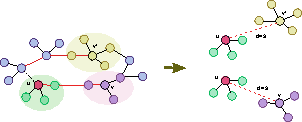
\includegraphics[width=0.9\columnwidth, height=4cm]{img/cdnk.pdf}
\caption{CDNK}
\label{fig:01}
\end{figure}

Formally, It defines two relations: the \textit{conjunctive relation} $R^{\wedge}_{r,d}(A_u, B_v, G_u)$ identical to the NSPDK relation $R_{r,d}(A_u, B_v, G)$,  and (ii) $\mathcal{D}(u,v)= d$; the \textit{disjunctive relation} $R_{r,d}^{\vee}(A_u, B_v, G_u)$ is true {\em iff} (i)  $A_u \cong \mathcal{N}_r^u$ and $B_v \cong \mathcal{N}_r^u$ are true, (ii) $\exists w$ s.t. $\mathcal{D}(w,v)= d$, and (iii) $(u,w)$ is a disjunctive edge. Besides, it defines $\kappa_{r,d}$ on the  inverse relations ${R^{\wedge}_{r,d}}^{ -1}$ and ${R^{\vee}_{r,d}}^{ -1}$ \vspace{8pt}\\

 $\kappa_{r,d}(G_u,G_{u'}) = \!\!\!\!\!\!\!\!\!\!\!\!
 \sum\limits_{\substack {A_u,{B}_{v} \in {R_{r,d}^{\wedge}}^{ -1}(G_u) \\ A'_{u'},{B'}_{v'} \in {R_{r,d}^{\wedge}}^{ -1}(G_{u'}) }} \!\!\!\!\!\!\!\!\!\!\!\!
  { \textbf{1}_{A_u \cong A'_{u'}} \cdot { \textbf{1}_{B_{v} \cong B'_{v'}}}}
+ \!\!\!\!\!\!\!\!\!\!\!\! \\
 \sum\limits_{\substack {A_u,{B}_{v} \in {R_{r,d}^{\vee}}^{ -1}(G_u) \\
  A'_{u'},{B'}_{v'} \in \ {R_{r,d}^{\vee}}^{ -1}(G_{u'}) }} \!\!\!\!\!\!\!\!\!\!\!\!
  { \textbf{1}_{A_u \cong A'_{u'}} \cdot { \textbf{1}_{B_{v} \cong B'_{v'}}}}
  $. \vspace{8pt}\\
The CDNK is finally defined as $K(G_u,G_v) = \sum\limits_{r}{\sum\limits_{d}{\kappa_{r,d}(G_u,G_v)}}$, where once again for efficiency reasons, the values of $r$ and $d$ are upper bounded to a given maximal $r^*$ and $d^*$.
\subsection{Disjunctive interconnection graph integration}
In this section, we first introduce the flow of our proposed method for disease gene prioritization. We then describe each part in detail.

We consider a set of graphs $\mathcal{G} = \lbrace g_1, g_,\ldots, g_n \rbrace$ where we refer each graph as a layer. Our method consists of following steps:
\begin{itemize}
\item Graph decomposition: Each graph is transformed into a collection of sparse sub-networks.
\item Graph labeling: Different ways are introduced to label for node and edges of each graph.
\item Graph union: we connect the set of graphs obtained from previous steps to form a single graph whose layers are linked with disjunctive links.
\item Similarity definition: we apply a particular graph node kernel, CDNK \cite{cdnk},  on the union graph to define node similarities which will be fed into a kernel machine to construct a model for disease gene inference.
\end{itemize} 

\begin{figure}[ht]
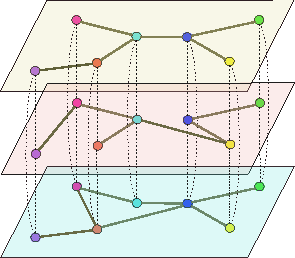
\includegraphics[width=0.9\columnwidth, height=6cm]{img/multilayers.pdf}
\caption{Graph Disjunctive Interconnection Illustration}
\label{fig:graph_interconnection}
\end{figure}

\subsection*{Graph Decomposition} 
\label{network-decomposition}
Graph decompositional kernels can only efficiently work on graphs whose nodes with low degree. However, it is common to find nodes with degree in gene-based networks. It prevents decompositional kernels from showing promising performance due to the high number of neighborhood subgraphs. To overcome this problem, in \cite{cdnk}, a network decomposition procedure is proposed with the aim of transforming a given network into a collection of sparse sub-networks whose \textit{conjunctive} links only are linked by \textit{disjunctive} links. The decompostion works by first applying the k-core decomposition iteratively and then the clique decomposition. Following we describe in detail each decomposition type in detail.

\textit{Iterative k-core decomposition}: The node set is partitioned in two groups on the basis of the degree of each node w.r.t. a threshold degree $D$. The node partition is used to induce the conjunctive vs disjunctive edge partition: edges that have endpoints in the same part are marked as conjunctive, while edges with endpoints in different parts are marked as disjunctive. We apply the k-core decomposition iteratively considering only the graph induced by the conjunctive edges until no node has a degree \footnote{The degree is defined by only considering incident conjunctive edges.}greater than $D$.

\begin{figure}[ht]
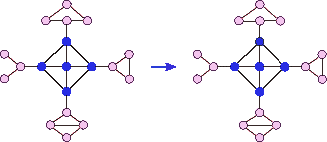
\includegraphics[width=0.9\columnwidth, height=3cm]{img/k_core.pdf}
\caption{K-core decomposition}
\label{fig:01}
\end{figure}

\textit{Clique decomposition}: To model the notion that nodes in a clique are tightly related, we summarize the whole clique with a new 'representative' node. All the cliques (completely connected subgraphs) with a number of nodes greater than a threshold size $C$ are identified. The endpoints of all edges incident on the clique's nodes are transferred to the representative node. Disjunctive edges are introduced to connect each node in the clique to the representative. Finally all edges with both endpoints in the clique are removed.
\begin{figure}[ht]
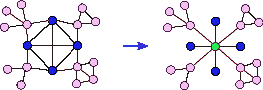
\includegraphics[width=0.9\columnwidth, height=2.5cm]{img/cliques.pdf}
\caption{Clique decomposition}
\label{fig:01}
\end{figure}
In our work a network is transformed by applying first the iterative k-core decomposition and then the clique decomposition.

\subsection*{Graph labeling}
\textbf{Node labeling}: we employ two methods to label for nodes in a graph. Both methods are based on the idea that genes with similar number of neighborhoods tend to have similar properties. We consider both conjunctive and disjunctive edges to compute the node degree.
\begin{itemize}
\item The first node labeling function, $\ell_1$, assigns the degree for nodes $u$ having degree less than or equal a user defined threshold $T$ ($T=5$ in our experimental evaluation). However degree values larger than $T$ are subsequently discretized into $k$ levels. Formally, the labeling function is defined as:
\begin{center}
$\ell_1(u) = \left\{
	\begin{array}{ll}
		deg(u),\  & \mbox{if } deg(u) \leq T \\
		T+i,\ & \mbox{if } deg(u) > T
	\end{array}
\right.$,
\end{center}
where $i = \lceil \frac{deg(u)-T}{bin}\rceil$, $bin = \frac{deg(G)-T}{\lambda - T}$ and $\lambda$ ($\lambda > T$) is the maximum number of symbols used. The value of $\lambda$ depends on the degree distribution and can be tuned as a hyperparameter of the approach.

\item The second node labeling function, $\ell_2$ implements the idea of equal frequency discretization. Given number of bins, $k$, we assign nodes into bins such that two criteria. First, nodes with similar degree are assigned into the same bin. Second, every bin needs to have similar number of nodes. We then use the bin ID as label for its nodes.
\end{itemize}

\noindent \textbf{Edge labeling}: We assign labels for every edges in a layer as its layer ID.

\subsection*{Graph union} 
Consider a layer tuple $g_i$, $g_j$ ($g_i, g_j \in \mathcal{G}$) and two nodes $u\in g_i,\ v \in g_j$ such that $u$ and $v$ are both represent for a same gene, we connect $u$ and $v$ by a disjuctive link. As the consequence, we achieve a graph $g$ whose nodes represeting same genes in all graph layers are linked by disjuctive links. Figure \ref{fig:graph_interconnection} is a visualization for our graph integration idea. 

\subsection*{Similarity definition}
We employ CDNK to define similarity for the similarity for any couple of genes. The similarity between two genes $g_i$ and $g_j$ is the summation of similarity of between their corresponding nodes on all layers.
\section{Experiments}
In order to evaluate the performance of our proposed method, we conduct two separate experiments. In the first experiment, \textit{cross-validation evaluation}, we desire to compare our method with state-of-the-are methods for disease gene prioritization in the first experiment, while we intend to compare the performance our proposed method with web-tools for disease gene identification in the second experiment, \textit{unbiased evaluation}. Following, we first describe data sources employed for our experiments, we then present the procedures to carry out them.

\subsection*{Data sources}
\begin{itemize}
	\item \textbf{Human Protein Reference Database} (\textbf{HPRD}): a database of curated proteomic information pertaining to human proteins. It is derived from \cite{hprd1} with 9,465 vertices and 37,039 edges. We employ the HPRD version used in \cite{hprd2} that contains 7311 nodes and 30503 edges. 	
	
	\item \textbf{BioGPS} \cite{biogps1, biogps2} a gene co-expression graph (7311 nodes and 911294 edges) constructed from the BioGPS dataset, which contains 79 tissues, measured with
the Affymetrix U133A array. Edges are inserted when the pairwise Pearson
correlation coefficient (PCC) between genes is larger than 0.5.	
	
	\item \textbf{Pathways}: Pathway datasets are obtained from the database of KEGG \cite{kegg}, Reactome \cite{reactome}, PharmGKB \cite{pharmgkb} and PID \cite{pid}, which contain 280, 1469, 99 and 2679 pathways, respectively. A pathway co-participation network is constructed by connecting genes that co-participate in any pathway.
	\item \textbf{String}: The String database gathers protein information covering seven levels of evidence: genomic proximity in procaryotes, fused genes, co-occurrence in organisms, co-expression, experimentally validated physical interactions, external databases and text mining. Overall, these aspects focus on functional relationships that can be seen as edges of a weighted graph, where the weight is given by the reliability of that relationship. To perform the unbiased evaluation we employed the version 8.2 of String \cite{string}, from which we extracted functional links among 17078 human genes.
	\item \textbf{Omim}: OMIM is a public database of disease-gene association. Genes
implicated in the same disease are more likely to be involved in other
similar diseases as well. Therefore, Omim network is formed by connecting genes which are involved in common disease(s).
\end{itemize}

\subsection*{Cross-validation evaluation} We follow the experimental setting used in \cite{f3pc}. In this experiment, three datasets are employed: BioGPS, HPRD and Pathways. To perform the experiment, 12 disease-gene associations are selected from OMIM data source with at least 30 confirmed genes. Concerning each disease, we construct a a positive set ($P$) which contains its all confirmed disease genes. For the negative set ($N$), we randomly sample from the set of genes which are related to at least one disease, but not with the disease that defines $P$, such that $|N| = \frac{1}{2}|P|$. 

For evaluation, a leave-one-out cross validation is used. Iteratively, each turn a gene in the training set ($P \cup N$) is selected to be the test gene and the remaining genes used to train the model. For each test gene $g_i$, the model returns a score $s_i$ proportional to the likelihood of being associated to the disease. Next a decision score $q_i$ is
computed as the top percentage value of $s_i$ among all candidate gene scores.
We collect all decision scores for every test genes to compute the area under
the curve for the receiver operating characteristic (AUC-ROC).

\subsection*{Unbiased evaluation} When a new gene-based discovery is made, most related data sources are updated. Therefore, the performance of methods evaluated through the previous experiment could be over-optimistic. To void this inflation, we conduct our experiment following the setting used in \cite{unbiased_evaluation} with the aim at comparing our method performance with different web tools for disease gene prioritization.
Newly discovered disease-gene associations were collected over a timespan of six months, gathering 42 associations. As soon as a new association was discovered, eight pre-selected gene prioritization web tools were queried with a proper training set in order to mimic the discovery through each of them. These 42 predictions were used to assess the ability of the tools to successfully prioritize disease genes. The idea behind this procedure is to anticipate the integration of the associations in the data sources and so avoid biased predictions.

To evaluate the performance of DIGI, we backdated our datasets to a time prior to May 15, 2010 by employing String v8.2 data \cite{string} and OMIM. The candidate sets were constructed by considering all genes with Ensembl \cite{ensembl} gene identifier within the chromosomal regions around the test genes, in order to get on average 100 candidates for each trial. Then, we performed prioritizations for each test gene in two distinct cases - genome-wide and candidate set-based prioritizations. In genome-wide prioritizations all coding genes in the genome were prioritized, while in candidate set-based tests only the genes belonging to the candidate groups were ranked. In both cases, we normalized ranking positions over the total number of genes in order to get the median and the standard deviation of the normalized ranks for test genes. We also computed the true positive rate (TPR) relatively to some representative thresholds (5\%, 10\% and 30\% of the ranking) and the AUC obtained by averaging over the 42 prioritizations.

\subsection*{Model Selection} The hyper-parameters of our method are set using a 3-fold on training set in which one fold is used for training the model and two remaining folds are used for validation. For CDNK, we try for the degree threshold value in $\lbrace 10,\ 15,\ 20 \rbrace$, clique size threshold in $\lbrace 4,\ 5 \rbrace$, maximum radius in $\lbrace 1,\ 2 \rbrace$, maximum distance in $\lbrace 2,\ 3,\ 4 \rbrace$. The number of bins, $k$, in node labling function $\ell_1$ and $\ell_2$ is set in $\lbrace 7, 10, 12 \rbrace$. Finally, the regularization tradeoff $C$ for the SVM is chosen in $\lbrace 10^{-4}, 10^{-3}, 10^{-2},\ 10^{-1}, 1,\ 10,\ 10^2, \\ 10^3,\ 10^4 \rbrace$.
\section{Results and discussion}
Table \ref{tab:unbiased_evalutation} and \ref{tab:cross_validation_evaluation} show the performance of our proposed method together with different methods and tools in unbiased evaluation and cross validation setting, respectively. Overall, DIGI outperforms all compared methods. 

In the Unbiased evaluation setting, it can be seen from the table \ref{tab:unbiased_evalutation} that our method shows impressive performance which considerably higher than other's in both cases: Genome-wide and candidate genes. In particular, It shows big difference with the second best one, Scuba, with around 15$\%$ higher in both top 5$\%$ and 10$\%$. For the time and finance constraints, we normally take genes at very top in the ranking to have further tests. Therefore, having high accuracy in top 5$\%$ and 10$\%$ is really meaningful in practice.
It is also competive in top 30$\%$ with 85.7$\%$ and 88.1$\%$ for Genome-Wide and Candidate-Genes, respectively. It only shows a bit lower, around 2$\%$, than Endeavour with 90.5$\%$ in Candidate-Genes. Similarly for AUC measure, it show the best results in both cases with 87 and 86. Concerning the median rank, a huge gap between our method and the rest of compared methods can be observed from the table. We also report the relative position over 42 genes in the rank of DIGI in Figure \ref{fig:histogram-genomewide} and \ref{fig:histogram-candidate} in the two cases.
We can see that most test genes are ranked in the top of the rank, especially 22 and 17 genes are in in top 5$\%$ with 22 and 17 genes for Genome-Wide and Candidate, respectively. There is only 1 gene for each case in a very low position, top 80$\%$ and 90$\%$.


In the Cross validation setting, DIGI together with Scuba show the best performance with high gaps, at least 4.6$\%$ difference, compared with the rest of methods. Between DIGI and Scuba, DIGI presents a slightly higer than Scuba with 88.1$\%$ and 87.6$\%$, respectively. The worse performance methods in this setting are DIR and GeneWanderer.

\begin{table*}[!htb]
\caption{Performance of DIGI comparing with Scuba and other web tools on unbiased setting} 
\label{tab:unbiased_evalutation}
\setlength\tabcolsep{0pt} % let LaTeX compute intercolumn whitespace

\centering
\smallskip 
\begin{tabular*}{\textwidth}{@{\extracolsep{\fill}}ccccccl}
\hline
  Tool/Method & Response & Rank & TPR in top & TPR in top & TPR in top & AUC\\
              & rate (\%)    & median (\%) & 5\% (\%) & 10\% (\%) & 30\% (\%) & (\%)\\
\hline
Genome-Wide \\  
  DIGI & 100 & \textbf{4.73} & \textbf{52.4} & \textbf{59.5} & \textbf{85.7} & \textbf{87} \\
  Scuba & 100 & 10.55  &  33.3 & 47.6 & 78.6 & 80 \\
  Candid & 100 &  18.10 & 21.4 & 33.3 & 64.3 & 73 \\
  Endeavour & 100 &  15.49 & 28.6 & 38.1 & 71.4 & 79 \\  
  Pinta & 100 & 19.03 & 26.2 & 31.0 & 71.4 & 77 \\
  \hline
  Candidate-Genes \\
  DIGI & 100 & \textbf{6.10} & \textbf{50.0} & \textbf{59.5} & 88.1 & \textbf{86} \\ 
  Scuba & 100 &  12.95  &  28.6 & 45.2 & 73.8 & 78 \\
  Suspects & 88.9$^a$ &  12.77$^a$ & 33.3$^a$ & 33.3$^a$ & 63.0$^a$ & 76$^a$ \\
  ToppGene & 97.6 &  16.80 & 35.7 & 42.9 & 52.4 & 66 \\  
  GeneWanderer-RW & 88.1 &  22.10 & 16.7 & 26.2 & 61.9 & 71 \\
  Posmed-KS & 47.6 &  31.44 & 4.7 & 7.1 & 23.8 & 58 \\
  GeneDistiller & 97.6 &  11.11 & 26.2 & 47.6 & 78.6 & 85\\  
  Endeavour & 100 &  11.16 & 26.2 & 42.9 & \textbf{90.5} & 82 \\
  Pinta & 100 & 18.87 & 28.6 & 31.0 & 71.4 & 75 \\  
\hline
\end{tabular*}
\end{table*}
%====================================

\begin{figure*}
\centering
\begin{minipage}{.5\textwidth}
  \centering
  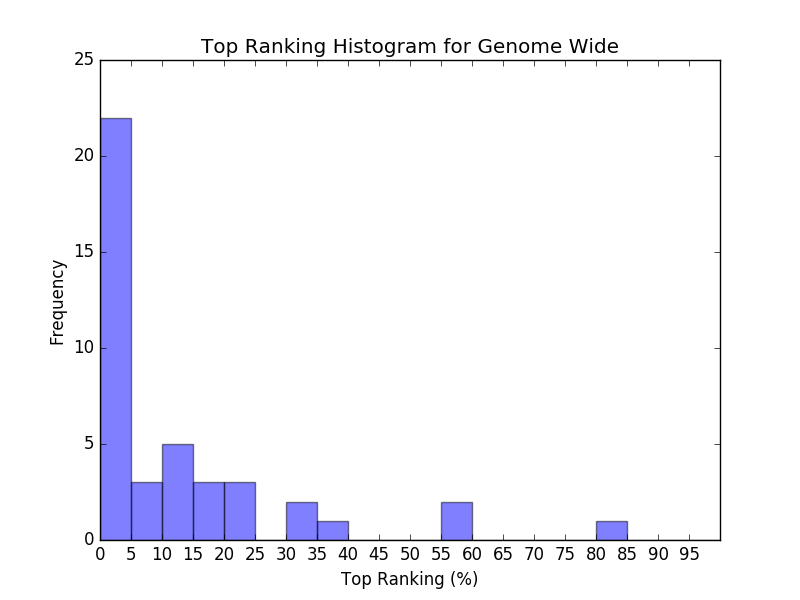
\includegraphics[width=1\linewidth]{img/histogram_genomewide.png}
  \caption{Top Rank Histogram for Genome-Wide Setting}
  \label{fig:histogram-candidate}
\end{minipage}%
\begin{minipage}{.5\textwidth}
  \centering
  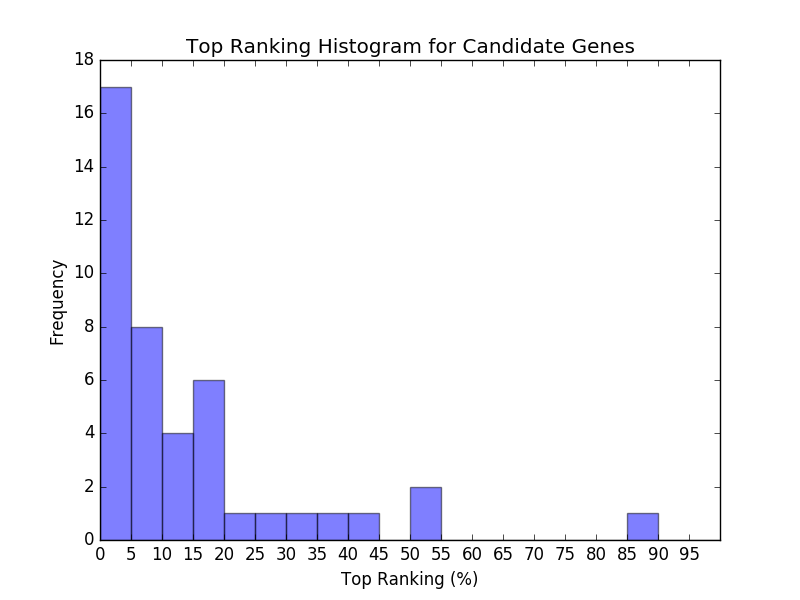
\includegraphics[width=1\linewidth]{img/histogram_candidate.png}
  \caption{Top Rank Histogram for Candidate Setting}
  \label{fig:histogram-candidate}
\end{minipage}
\end{figure*}



%====================================
\begin{table}[!htb]
%\setlength\tabcolsep{10pt} % let LaTeX compute intercolumn whitespace
%\centering
%\smallskip 
\caption{Performance of different methods on Cross validation setting} \label{tab:cross_validation_evaluation}
\centering
\begin{tabular}{cc}
\hline
  Method  & ROC-AUC (\%) \\
\hline
  DIR & 71.6 \\
  F3PC & 83.0 \\
  MRF & 73.1 \\
  GeneWanderer & 71.1 \\
  Scuba & 87.6 \\
 \textbf{DIGI} & \textbf{88.1} \\
\hline
\end{tabular}
\end{table}
\section{Conclusion}
We have proposed an efficient method for graph integration for disease gene prioritization. In our method, first graph layers are decomposed and disjunctively interconnected to let information traversing between layers. It then employ a perticular graph node kernel, which is able to efficiently exploit the graph structure resulted from the graph integration paradigm, to compute the capture the node similarities. As a consequence, it shows promissing performance and outforms all methods/tools employed in two experimental setttings.
\chapter{Conclusion and Future Work}
\bibliography{thesisBib}{}
\bibliographystyle{plain}
\appendix
\input{appendix.tex}
\end{document}
